\documentclass[11pt]{article}
\usepackage{fontspec}
\usepackage{luatexja-fontspec}\setmainjfont[BoldFont=FandolSong-Bold.otf,ItalicFont=FandolKai-Regular.otf]{FandolSong-Regular.otf}
\setsansjfont[BoldFont=FandolHei-Bold.otf]{FandolHei-Regular.otf}
\usepackage[letterpaper,margin=1.03in]{geometry}
\usepackage{amsmath,amssymb,amsthm,mathtools,bm}
\usepackage{graphicx,booktabs,enumitem,float,tabularx}
\usepackage[numbers,sort&compress]{natbib}
\usepackage{placeins}
\usepackage[colorlinks=true,citecolor=blue!55!black,linkcolor=blue!50!black,urlcolor=blue!55!black]{hyperref}
\usepackage{xcolor}
\usepackage{caption}
\captionsetup{font=small,labelfont=bf}\renewcommand{\figurename}{图}\renewcommand{\tablename}{表}\renewcommand{\abstractname}{摘要}\renewcommand{\refname}{参考文献}\renewcommand{\proofname}{证明}
\setlength{\parindent}{1.2em}
\setlength{\parskip}{0.16em}
\setlength{\emergencystretch}{1em}
\numberwithin{equation}{section}
\newtheorem{theorem}{定理}[section]
\newtheorem{proposition}[theorem]{命题}
\newtheorem{corollary}[theorem]{推论}
\newtheorem{lemma}[theorem]{引理}
\theoremstyle{definition}
\newtheorem{definition}[theorem]{定义}
\newtheorem{assumption}[theorem]{假设}
\theoremstyle{remark}
\newtheorem{remark}[theorem]{注}
\hypersetup{pdftitle={市场何时会在没有新闻的情况下崩盘？},pdfauthor={Siyuan Ye},pdfsubject={特定模型下的系统性回撤可达性理论}}
\newcommand{\R}{\mathbb{R}}
\newcommand{\Cris}{\mathcal{C}}
\newcommand{\calK}{\mathcal{K}}
\newcommand{\calA}{\mathcal{A}}
\newcommand{\dd}{\,\mathrm{d}}
\newcommand{\one}{\mathbf{1}}
\newcommand{\pos}[1]{[#1]_+}
\newcommand{\Law}{\mathcal{L}}
\newcommand{\totv}{\operatorname{TV}}
\title{\textbf{市场何时会在没有新闻的情况下崩盘？}}
\author{Siyuan Ye\\{\small 独立研究者}}
\date{2026 年 10 月}
\begin{document}
\maketitle
\begin{center}\footnotesize 完整简体中文译本，经作者授权公开。数学内容以英文 V12 Final 原文为准。译稿日期：2026-10-15；版权保持原有声明。\end{center}
\vspace{-0.95em}
\begin{abstract}\noindent
在基本面固定、实行成交金额配对执行的韧性 $N$ 资产市场中，我们证明：响应弹性 $e(S)=Sg'(S)/g(S)\ge2$ 排除一切正的系统性回撤，而 $e(S)\ge1$ 排除所有资产同时下跌。证明采用响应适配广义价格坐标 $\Phi(S)=\int_F^S u/g(u)\,\mathrm{d}u$，其唯一归一化使成交美元转移产生等量的坐标位移。这揭示了可加的交易守恒律及由恢复驱动的稳定性屏障。在统一函数族 $g_p(S)=\eta(S/F)^p$ 中，$p=2,1,0$ 三种情形依次产生排除、受库存约束的部分覆盖损失，以及允许脉冲时在统一有限换手与库存下任意严重的部分覆盖对数损失。我们建立必要的美元换手和股数库存界。对于恒定每股冲击和有界毛成交股数速率，低速率下最大的系统性损失为二次阶，并给出达到该阶的连续构造。滚动每日价格限制约束单个交易时段，却未必排除多日损失：一条计算机辅助验证的十资产路径使九项资产在连续两个时段收于跌停价，逐项闭合所有成交美元账簿，并实现超过 $0.020$ 的系统性对数损失。本例所需的毛成交速率上限满足 $0.044<\bar v_*<0.285$。
\end{abstract}
\noindent\textbf{关键词：} 市场崩盘；价格冲击；市场韧性；系统性回撤；可达性；执行约束。\par
\noindent\textbf{MSC 2020:} 91G15, 91G45, 93B03, 65G30, 91G80.

\section{引言}\label{sec:intro}
市场大幅下跌未必源于坏消息。交易本身改变边际价格，市场韧性则决定这种位移能够保留多少。因此，一个基本而影响深远的问题是：遵守市场自身结算规则的交易，能否迫使基本面不变的市场发生\emph{广泛的共同损失}？我们提出的问题比均衡如何选择崩盘更为狭窄：\emph{哪些系统性损失状态是可达的，到达这些状态需要哪些实际成交的交易资源？}

现有研究通过不同市场机制解释无新闻的价格变动。Gennotte 和 Leland~\citep{GennotteLeland1990} 分析动态对冲与推断，Romer~\citep{Romer1993} 研究没有外部新闻时交易所揭示的信息。Huang 和 Wang~\citep{HuangWang2009} 说明非同步交易需求如何产生内生订单失衡；Cespa 和 Foucault~\citep{CespaFoucault2014} 描述跨资产流动性的反馈。在相关的多资产环境中，Cont 和 Wagalath~\citep{ContWagalath2013} 从困境抛售推导内生收益依赖关系。这些模型说明流动性驱动的不稳定性为何重要。我们研究一个互补的数学问题：\emph{哪些共同终端损失与给定的执行规律、恢复动态及每项资产终端成交美元账簿归零相容？}

Kyle~\citep{Kyle1985} 的均衡价格响应基准是一个经典起点。价格冲击与恢复模型为定量研究这一问题提供工具。Obizhaeva 和 Wang~\citep{ObizhaevaWang2013}、Alfonsi 和 Schied~\citep{AlfonsiSchied2010} 刻画韧性流动性下的交易执行；Gatheral~\citep{Gatheral2010}、Alfonsi、Schied 和 Slynko~\citep{AlfonsiSchiedSlynko2012} 以及 Huberman 和 Stanzl~\citep{HubermanStanzl2004} 从交易成本与操纵准则推导限制。Alfonsi、Kl\"ock 和 Schied~\citep{AlfonsiKlockSchied2016} 分析多元暂态冲击，Cordoni 和 Lillo~\citep{CordoniLillo2024} 研究多主体、多资产冲击博弈中的均衡不稳定性。Kyle 和 Obizhaeva~\citep{KyleObizhaeva2023} 通过市场微观结构不变性，将大额头寸与执行速度联系到观测到的崩盘。我们以这些机制为动机，开展另一项工作：在指定结算协议下刻画\emph{可行的系统性损失状态}，继而量化通向这些状态的路径所受换手、库存、速率及价格区间约束。

我们研究一个\emph{无现金风险资产再配置池}：每笔成交卖出都与等美元金额的风险资产买入配对，每项资产的终端带符号美元流量均为零。价格向固定基准 $F$ 恢复，成交股数则通过正响应函数 $g(S)$ 改变边际价格。关键步骤是在\emph{响应适配坐标}中衡量价格，使成交美元原本非线性的作用变为可加作用。成对交易因而保持这些坐标之和不变；韧性在交易间改变其总和。坐标曲率产生排除屏障，并在共同约束下统一三种响应情形。随后，我们考察加入执行资源与交易所限制后，结构上允许的哪些损失仍然可达。

在毛成交股数速率有界且设有每日价格区间时，可达性要求不止一个获准的价格终点。当大多数资产下跌时，其余资产必须接收配对美元，但它们的价格与执行速率同样受到约束；此外，它们的升值可能抵消危机准则中的平均损失。我们推导必要速率界与跨子集容量界，并验证一条明确的两日路径，其中十项资产中的九项反复收于简化的跌停价。所得结果是满足全部规定路径约束的\emph{经认证多日系统性回撤见证}，为必要资源不等式提供明确的存在性对应结果。

我们的分析从结构屏障推进到必要资源，再从执行限制推进到同时满足约束的可行性证书。以下先给出主要结论，随后给出共同市场定义与证明。

\begin{theorem}[主要结果（非正式表述）]\label{thm:informal}
在第~\ref{sec:model} 节定义的成交金额配对韧性市场中，成立以下结论。
\begin{enumerate}[label=\textup{(\roman*)},leftmargin=2em,itemsep=0.12em]
\item \emph{结构性排除。} 若在所有容许价格上 $e(S)=Sg'(S)/g(S)\ge2$，则对任意覆盖广度和时刻均有 $\Cris_\alpha(t)\le0$。较弱条件 $e(S)\ge1$ 排除所有资产同时下跌。
\item \emph{可达性情形。} 对于 $g_p(S)=\eta(S/F)^p$，$p=2,1,0$ 分别产生排除、受库存约束的部分覆盖回撤，以及在 $k=\lceil\alpha N\rceil<N$、有限期限足够长且允许脉冲时，在固定有限换手与库存上限下任意严重的部分覆盖损失。对于恒定冲击及 $k=N$，依赖期限的锐界取代不受限制的严重程度。
\item \emph{执行资源。} 一般正函数 $g$ 给出明确的必要美元换手与股数库存界。在恒定每股冲击及有界毛成交股数速率下，低速率危机界为二次阶，且连续美元闭合构造能够达到此阶。
\item \emph{多日执行。} 滚动价格区间限制每个时段的损失，速率限制与接收资产容量则限制连续收于跌停价。计算机辅助验证的两日十资产路径满足这些控制，九项资产连续两次收于跌停价，并产生 $\Cris_{0.9}(T)>0.020$；该实例满足 $0.044<\bar v_*<0.285$。
\end{enumerate}
\end{theorem}

共同的数学工具是\emph{响应适配广义价格坐标}
\begin{equation}\label{eq:phi-intro}
\Phi(S)=\int_F^S\frac{u}{g(u)}\dd u.
\end{equation}
在该坐标中，一美元成交产生一单位价格状态位移。成对交易中的可加守恒，加上交易间的恢复漂移，将结构屏障与资源及多日执行结果联系起来。

\section{市场：假设、执行与价格动态}\label{sec:micro}\label{sec:model}
我们规定一个风险资产再配置子市场，每笔成交卖出均匹配等美元金额的买入。结算与价格响应是不同的假设：前者约束流量，后者决定所诱发的价格运动。后续全部定理采用同一市场定义。

\begin{assumption}[成交金额配对韧性市场]\label{asmp:model}
固定 $N\ge2$ 项资产与有限期限 $[0,T]$。以下条件共同定义容许市场。
\begin{enumerate}[label=\textup{(M\arabic*)},leftmargin=2.9em,itemsep=0.20em]
\item \textbf{正价格与坐标。} 每个成交价格 $S_i(t)$ 严格为正，初始满足 $S_i(0)=F>0$。严格递增的 $C^1$ 坐标 $q_i=\phi_i(S_i)$ 保持价格优先顺序。本分析研究确定性的容许执行路径。
\item \textbf{交易与执行核算。} 成交股数变动为带符号量 $\dd\theta_i$；无符号成交量计入其绝对增量，不将交易双方重复计数。成交遵循边际价格结算 $\dd X_i=S_i\dd\theta_i$。撮合在给定订单簿条件下采用价格优先；有效价格响应则为另行规定的正的局部 $C^2$ 函数 $g(S)$，使得 $\dd S_i|_{\rm trade}=g(S_i)\dd\theta_i$。
\item \textbf{无基本面新闻与韧性。} 基准 $F$ 保持固定。交易间价格向 $F$ 恢复，共同常数速率为 $\rho>0$：无成交时 $\dot S_i=-\rho(S_i-F)$。响应函数 $g$ 与 $\rho$ 是\emph{模型输入}，并非价格优先的推论。
\item \textbf{成交金额配对交易网络。} 每笔获准交易在来源资产与目标资产之间转移等额成交美元：$\dd\bm X=B\dd\bm z$，其中 $B$ 为完全双向图的有向关联矩阵，$\dd\bm z\ge0$，且 $\one^\top B=0$。这描述所选的成对再配置子市场；主动订单压力零和并非所有真实市场的普遍事实。
\item \textbf{容许控制与终端闭合。} 路径分段连续且具有有限执行变差，允许有限多个按边际价格结算的瞬时脉冲；所有价格保持为正，所需卖出库存均可在无卖空条件下提供。终端比较对\emph{每项}资产施加 $X_i(T)=0$，而非 $\theta_i(T)=\theta_i(0)$。凡提出资源上限的情形，各市场均采用相同的配对成交金额总换手与每项资产初始股数限制。
\end{enumerate}
\end{assumption}



\paragraph{美元账簿为何闭合。}
(M4) 中的完全双向图表示理想化的投资组合切换池，或成交卖出所得必须立即用于买入其他风险资产的无现金再配置组合。这不是一般全交易所订单流的恒等式：在普通股票市场中，现金账户或额外交易对手可以吸收卖出所得。我们施加更强的终端条件 $X_i(T)=\int_0^T S_i\,\dd\theta_i=0$，以研究\emph{每项}资产的一阶净美元再配置抵消后剩余的价格位移。这是一项研究归一化，并非交易往返的通常定义。股数持平的往返交易要求 $\theta_i(T)=\theta_i(0)$，两种约束的含义不同。特别地，由下文 \eqref{eq:cost} 可知，具有终端位移或正恢复耗散的美元闭合要求消耗初始可用的股数库存：$F[\theta_i(0)-\theta_i(T)]=E(S_i(T))+\rho\int_0^T(S_i-F)^2/g(S_i)\,\dd t$。终点净成交金额闭合不恢复股数。这一区别对屏障结果至关重要。

\paragraph{有限变差路径与边际结算脉冲。}
对于绝对连续控制，微分记号具有经典意义。在跳跃处，我们\emph{不}采用左端点或右端点 Stieltjes 乘积 $S_i\Delta\theta_i$。相反，固定物理时间，每条有向边 $e:i\to j$ 承载美元质量 $z>0$，沿规定的事件内部参数 $a\in[0,z]$ 执行：
\begin{equation}\label{eq:pulse-flow}
\frac{\dd \widetilde S_i}{\dd a}=-\frac{g(\widetilde S_i)}{\widetilde S_i},\quad
\frac{\dd \widetilde S_j}{\dd a}=\frac{g(\widetilde S_j)}{\widetilde S_j},\quad
\frac{\dd\widetilde\theta_i}{\dd a}=-\frac{1}{\widetilde S_i},\quad
\frac{\dd\widetilde\theta_j}{\dd a}=\frac{1}{\widetilde S_j}.
\end{equation}
所得端点流量满足 $\Delta X_i=-z$、$\Delta X_j=z$ 以及 $\Delta\Phi(S_i)=-z$、$\Delta\Phi(S_j)=z$。等价地，单股脉冲通过求解 $\dd\widetilde S/\dd\xi=g(\widetilde S)$，并沿响应轨迹积分 $\int\widetilde S\,\dd\xi$ 来计算。因此，跳跃是保留普通链式法则的\emph{流补全}（Marcus 型）更新。不同边上的有限脉冲按规定顺序处理。仅当全部中间价格严格为正时，脉冲才容许。这些规则规定下文所有跳跃表达式的含义。

\paragraph{从条件撮合映射到有效响应。} 固定一个冻结订单簿 $\mathcal B$，其局部股数深度密度 $\rho_S(S;\mathcal B)$ 连续且为正。带符号边际股数为 $\dd\theta$ 的单边扫单遵循局部关系
\begin{equation}\label{eq:frozen-depth}
\dd\theta=\rho_S(S;\mathcal B)\dd S,
\qquad \rho_q(q;\mathcal B)\dd q=\rho_S(S;\mathcal B)\dd S.
\end{equation}
精确的离散版本使用订单簿累计深度的广义逆。在连续近似中，改变 $q=\phi(S)$ 通过雅可比改变密度的数值，而不改变撮合优先顺序。该关系针对边际成交价格。动态中间价、补充后的订单簿及资产间交叉冲击\emph{不能}由坐标变换推导。相反，假设 (M2) 在本文其余部分选择 $g(S)=1/\rho_S^{\rm eff}(S)$ 作为依赖状态的\emph{有效}响应。

\paragraph{所得 $N$ 资产方程。} 在完整市场设定下，价格水平方程为
\begin{equation}\label{eq:level-dynamics}
\boxed{\dd S_i(t)=-\rho\big(S_i(t)-F\big)\dd t+g(S_i(t))\dd\theta_i(t),\qquad \dd X_i=S_i\dd\theta_i.}
\end{equation}
选择严格单调广义坐标 $q_i=\log(S_i/F)$。转换为成交金额配对得到
\begin{equation}\label{eq:log-impact}
\dd q_i\big|_{\rm trade}=\frac{g(S_i)}{S_i^2}\dd X_i.
\end{equation}
结合这一转换、交易配对及韧性，得到完整多资产系统
\begin{equation}\label{eq:master}
\boxed{\dd\bm q=-\rho(\one-e^{-\bm q})\dd t+D(\bm q)B\dd\bm z,\qquad
D_{ii}(\bm q)=\frac{g(Fe^{q_i})}{F^2e^{2q_i}}.}
\end{equation}
指数按分量作用。该对数坐标便于衡量损失，但成交美元允许使用更简单的\emph{响应适配}坐标。令 $y_i=\Phi(S_i)$，其中 $\Phi$ 由~\eqref{eq:phi-intro} 给出。它严格递增且满足 $\Phi(F)=0$。此外，在可微坐标 $\psi$ 中，采用归一化 $\psi(F)=0$ 后，要求每笔边际交易满足 $\dd\psi(S)|_{\rm trade}=\dd X$，强制给出 $\psi'(S)g(S)=S$，因而唯一选定 $\psi=\Phi$。定义恢复响应
\[
\mathcal R(y)=\frac{S(S-F)}{g(S)},\qquad S=\Phi^{-1}(y).
\]
于是整个多资产市场具有\emph{交易归一化形式}
\begin{equation}\label{eq:normal-form}
\boxed{\dd\bm y=B\dd\bm z-\rho\mathcal R(\bm y)\dd t,\qquad\one^\top B=0,}
\end{equation}
其中 $\mathcal R$ 按分量作用，执行规则也适用于流补全脉冲。因此，交易是可加的零和输入；所有非线性价格状态依赖都进入恢复项及逆映射 $S=\Phi^{-1}(y)$。变换后的状态空间是 $\mathcal J^N$，其中 $\mathcal J=\Phi((0,\infty))$。对于 $g_p(S)=\eta(S/F)^p$，值域依次为 $(-F^2/[\eta(2-p)],\infty)$（当 $p<2$ 时）、$\mathbb R$（当 $p=2$ 时）及 $(-\infty,F^2/[\eta(p-2)])$（当 $p>2$ 时）。因此，可加交易输入并未消除严格正价格要求或执行约束。这一坐标变换不改变哪些价格状态可达。当 $\rho=0$ 时，交易的广义坐标之和精确守恒。

\begin{definition}[终端系统性回撤]\label{def:crash}
令 $L_i(T)=\log[F/S_i(T)]$ 及 $\overline L(T)=N^{-1}\sum_i L_i(T)$。第 $k$ 大损失的序号满足 $k=\lceil\alpha N\rceil$，将该损失记为 $Q_\alpha(T)$。定义
\begin{equation}\label{eq:crash}
\boxed{\Cris_\alpha(T)=\min\{\overline L(T),Q_\alpha(T)\}.}
\end{equation}
对于 $\delta>0$，当 $\Cris_\alpha(T)\ge\delta$ 时发生\emph{终端危机}。因此，平均损失和至少 $k$ 项个体损失均必须达到 $\delta$。目标的选取独立于价格响应函数。
\end{definition}

离散覆盖规则具有实质意义：对于 $N=3$，$\alpha=0.9$ 意味着 $k=3$，因此要求全部三项资产下跌。更一般地，$k=N$ 与 $k<N$ 的区别决定补偿资产是否存在。这一区别首先出现在 A/B/C 分类中，随后出现在多日跨资产容量不等式中。首次到达事件 $\tau_{\alpha,\delta}=\inf\{t:\Cris_\alpha(t)\ge\delta\}$ 与美元闭合下的\emph{终端}危机不同；我们研究后者。

\begin{definition}[换手、股数库存与终端临界预算]\label{def:budget}
对容许路径 $\gamma$，令
\begin{equation}\label{eq:resource}
M(\gamma)=\sum_e\int_0^T\dd z_e,\qquad
H_i^-(\gamma)=\int_0^T\big(-\dd\theta_i\big)_+.
\end{equation}
在允许的初始库存 $H_i$ 及终点净成交金额闭合条件下，定义
\begin{equation}\label{eq:minbudget}
M_*^{\rm end}=\inf\{M(\gamma): X_i(T)=0\ \forall i,\ \Cris_\alpha(T)\ge\delta,\ \gamma\text{ admissible}\},
\end{equation}
约定 $\inf\varnothing=+\infty$。一笔成交金额配对转移在 $M$ 中仅计一次，尽管它在两项资产账簿中以相反符号出现。
\end{definition}

\paragraph{无获利往返交易性质的精确定义。} 定义
\begin{equation}\label{eq:E}
E(S)=\int_F^S\frac{u-F}{g(u)}\dd u\ge0.
\end{equation}
对任意从 $F$ 出发的容许路径，执行成本恒等式为
\begin{equation}\label{eq:cost}
\boxed{\int_0^T S_i\dd\theta_i=F[\theta_i(T)-\theta_i(0)]+E(S_i(T))
+\rho\int_0^T\frac{(S_i-F)^2}{g(S_i)}\dd t.}
\end{equation}
因此，\emph{股数持平}的往返交易在 (M2)--(M3) 下具有非负执行成本。本文的终端条件 $X_i(T)=0$ 闭合的是成交\emph{美元}而非股数：终端美元持平路径可能消耗初始库存。附录~\ref{app:accounting} 证明该核算恒等式及其对容许控制的推论。

\paragraph{与股数持平交易的比较。}
终端美元条件与标准股数持平条件不能互换。例如，当 $g\equiv\eta$ 时，单资产交易先买入充分小的 $a>0$ 股（在时刻 $0$），再卖出 $a$ 股（在时刻 $T$），于是满足 $\theta(T)=\theta(0)$，但终端价格为 $S(T)=F-\eta a(1-e^{-\rho T})<F$；其净成交美元不为零，\eqref{eq:cost} 中的正成本通过现金账户支付。反之，在 (M4) 下，若要求每项资产\emph{既}股数持平\emph{又}终端美元持平，将强制 $\sum_i[E(S_i(T))+\rho\int_0^T(S_i-F)^2/g(S_i)\,\dd t]=0$。因此，两种闭合同时成立时，不可能存在持续正时间的耗散性价格偏离。美元持平协议有意分离出一个不同于标准股数往返执行的经济问题。

\section{市场崩盘的结构屏障}\label{sec:barriers}
规范形~\eqref{eq:normal-form} 给出交易过程中的一个守恒标量。记 $H(\bm S)=\one^\top\bm y=\sum_i\Phi(S_i)$。对资产求和会抵消所有配对美元转移，仅余恢复项：
\begin{equation}\label{eq:potential-law}
\boxed{\dd H=-\rho\sum_{i=1}^N\mathcal R(y_i)\dd t
=-\rho\sum_{i=1}^N\frac{S_i(S_i-F)}{g(S_i)}\dd t.}
\end{equation}
标量 $H$ 是交易不变量，而非完整恢复动态下的守恒量。恢复漂移能否使 $H$ 穿过危机边界，取决于 $\Phi$ 的曲率。
引入响应弹性
\begin{equation}\label{eq:elasticity}
e(S)=\frac{Sg'(S)}{g(S)}.
\end{equation}
$\Phi$ 与 $G(x)=\Phi(Fe^x)$ 的导数为
\begin{equation}\label{eq:curvature}
\Phi''(S)=\frac{1-e(S)}{g(S)},\qquad
G''(x)=\frac{S^2}{g(S)}\,[2-e(S)],\quad S=Fe^x.
\end{equation}
两种曲率之差对应系统性损失的定义。阻止\emph{每项资产}低于自身基准的屏障，弱于阻止本文泛函为正的屏障，因为后者还涉及\emph{平均}对数损失。因此，同一坐标可以产生两个不同的排除命题。


\begin{theorem}[所有资产共同下跌的屏障]\label{thm:barrier1}
若在容许路径能够到达的所有价格上 $e(S)\ge1$，则 $S_i(t)<F$ 对每个 $i$ 同时成立的情形，在任何时刻 $t$ 都不可能发生。特别地，$k=N$ 时不存在可达的正危机。
\end{theorem}
\begin{proof}
式~\eqref{eq:curvature} 使 $\Phi$ 为凹函数。其在 $S$ 处的切线不等式为 $\Phi(F)\le\Phi(S)+\Phi'(S)(F-S)$，因此 $(S-F)\Phi'(S)\le\Phi(S)$。于是 \eqref{eq:potential-law} 给出交易间 $\dot H\ge-\rho H$；脉冲保持 $H$ 不变。由于 $H(0)=0$，比较得到 $H(t)\ge0$。若所有 $S_i(t)<F$，严格单调性及 $\Phi(F)=0$ 则反而意味着 $H(t)<0$，矛盾。
\end{proof}

\begin{theorem}[任意覆盖广度系统性危机的屏障]\label{thm:barrier2}
若在容许价格范围上 $e(S)\ge2$，则对每个容许控制、$N\ge2$、$\alpha\in(0,1]$ 及 $t\in[0,T]$，
\begin{equation}\label{eq:no-crash}
\boxed{\Cris_\alpha(t)\le0.}
\end{equation}
因此不能到达任何严格为正的系统性终端危机阈值。
\end{theorem}
\begin{proof}
前一定理给出 $H(t)\ge0$。\eqref{eq:curvature} 的第二个恒等式使 $G(x)=\Phi(Fe^x)$ 为严格递增凹函数。Jensen 不等式给出
\[
0\le\frac{H(t)}N=\frac1N\sum_iG(q_i(t))
\le G\!\left(\frac1N\sum_iq_i(t)\right).
\]
由于 $G(0)=0$ 且 $G$ 严格递增，故 $\sum_iq_i(t)\ge0$。因此平均损失 $\overline L(t)=-N^{-1}\sum_iq_i(t)$ 非正；定义~\ref{def:crash} 蕴含 \eqref{eq:no-crash}。
\end{proof}

这两个定理识别出在各自假设下\emph{任何}容许交易计划均无法到达的状态。它们是全局\emph{充分}条件，并非逆命题，也非稳定性的必要条件。若不等式仅在 $F$ 附近成立，则排除结果仅在整条路径停留于该邻域时适用；有限库存、交易连接或时间可能形成额外屏障。因此，下一问题是构造性的：\emph{放宽结构条件是否确实改变可达集？} A/B/C 比较在同一响应族内回答此问题，而不把充分条件失效解释为崩盘的证明。

\section{共同约束下的三种市场情形}\label{sec:regimes}
上述曲率条件确定哪些情形被禁止，但并未说明不等式失效时哪些情形成为可能。为在匹配的假设而非互不相关的模型下呈现区别，我们仅改变以下函数族中的响应形状
\begin{equation}\label{eq:power}
 g_p(S)=\eta\left(\frac SF\right)^p,\qquad p\in\{2,1,0\},\quad \eta>0.
\end{equation}
三个市场具有相同的 $N,T,F,\rho,\eta$、相同的初始价格及初始\emph{冲击}、相同的成交金额配对交易网络；数值比较时还具有相同的换手与库存上限。它们仅在指数 $p$ 上不同。在对数美元方程 \eqref{eq:master} 中，
\begin{equation}\label{eq:powerd}
 D_{ii}^{(p)}(q_i)=\frac\eta{F^2}e^{(p-2)q_i},\qquad e(S)=p.
\end{equation}
同一坐标公式对每个指数均可显式积分：
\[
\Phi_p(S)=\begin{cases}
\displaystyle \frac{F^p}{\eta(2-p)}\big(S^{2-p}-F^{2-p}\big),&p\ne2,\\[4pt]
\displaystyle \frac{F^2}{\eta}\log(S/F),&p=2.
\end{cases}
\]
因此，成对交易保持某个量不变，该量分别正比于 $\sum_iS_i^2$、$\sum_iS_i$ 或 $\sum_i\log S_i$，对应于 $p=0,1,2$。恢复在交易间改变这些量。图~\ref{fig:response} 展示对应的每美元成交瞬时响应：在 $F$ 以下，$p=0$ 响应对美元交易的放大最强。

\begin{figure}[t]
\centering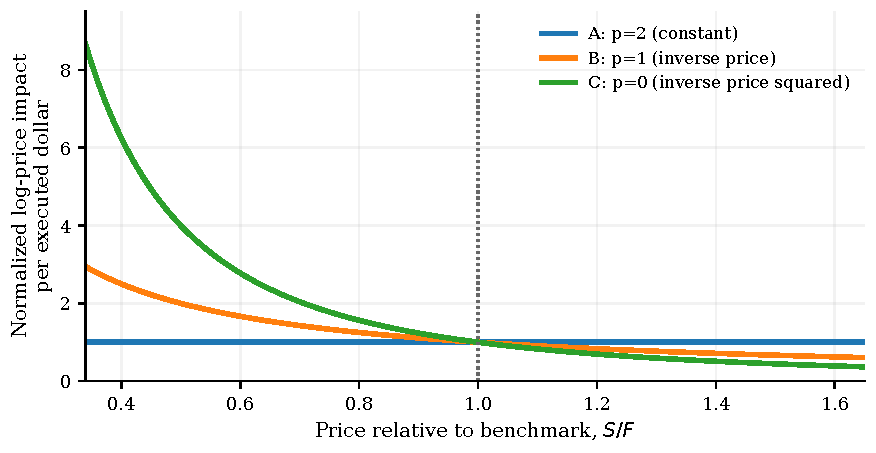
\includegraphics[width=0.82\linewidth]{../../paper/figures/response_regimes.pdf}
\caption{\textbf{一个响应函数族，三种价格敏感性。} 图中展示模型隐含的瞬时\emph{每美元成交对数价格变动}，并以共同初始值归一化。所有曲线在 $S=F$ 处重合。这是理论比较，并非对观测订单簿的拟合。}\label{fig:response}
\end{figure}

\begin{theorem}[A/B/C 可达性情形]\label{thm:ABC}
设 $N\ge2$ 及 $k=\lceil\alpha N\rceil<N$。在相同模型协议下比较 \eqref{eq:power} 中的三个市场。
\begin{enumerate}[label=\textup{(\Alph*)},leftmargin=2em,itemsep=0.15em]
\item \textbf{屏障市场（$p=2$）：} 对每条容许路径及任意期限，均有 $\Cris_\alpha(t)\le0$。
\item \textbf{库存有界市场（$p=1$）：} 正的但充分小的终端系统性回撤可达。若每项资产初始具有固定有限库存上限 $H_0$，且禁止卖空，则终端危机严重程度具有独立于交易序列的上界。
\item \textbf{严重损失可达市场（$p=0$）：} 对每个固定的 $N\ge2$ 及 $k<N$，存在充分长但有限的期限 $T$ 与有限常数 $M_0,H_0$，使得对\emph{每个}有限 $\delta>0$，均有满足 $M\le M_0$、$H_i^-\le H_0$ 及 $X_i(T)=0$ 的容许正价格路径达到 $\Cris_\alpha(T)>\delta$。
\end{enumerate}
(C) 中的常数可以依赖 $N,T,F,\rho,\eta$，但不依赖 $\delta$。当 $N\to\infty$ 时，它们不保持一致有界。
\end{theorem}
\begin{proof}
(A) 由定理~\ref{thm:barrier2} 得出。(B) 由命题~\ref{prop:two-pulse} 的双脉冲构造及下文库存不等式 \eqref{eq:inventoryb} 得出。(C) 在附录~\ref{app:severe} 中构造性地建立：$N-1$ 项目标资产被推动到任意接近零，同时一项资产充当现金流补偿者。该控制使用正价格、完全成对的边际美元成交、恢复时间的划分及每个 $X_i$ 的终端闭合。其显式换手与库存界独立于目标终价 $\varepsilon\downarrow0$。
\end{proof}

在相同成交美元及恢复协议下，三个响应函数产生不同的可达状态几何。市场 A 提供全局不变区域屏障；市场 B 说明库存有限时，非零部分覆盖损失并不必然意味着任意严重的损失；市场 C 则给出受控严重损失见证。(C) 中的 $k<N$ 至关重要：至少必须有一项资产承载补偿流量。施加有限毛成交股数速率后，这将成为明确的\emph{容量}约束，而不只是存在性要求。

对于 $p=1$，\eqref{eq:E} 中的库存势函数为
\begin{equation}\label{eq:inventoryb}
E_1(Fe^{-L})=\frac{F^2}{\eta}\left(L+e^{-L}-1\right).
\end{equation}
由 \eqref{eq:cost}，终点净成交金额闭合与禁止卖空蕴含 $E_1(S_i(T))\le FH_0$。由于 $L+e^{-L}-1\to\infty$（当 $L\to\infty$ 时），固定有限库存无法支持所需 $k$ 项资产的任意严重损失。相反，对于 $p=0$，$E_0(S)=(S-F)^2/(2\eta)$ 在 $S\downarrow0$ 时仍有界；这使 (C) 的构造成为可能，但本身并不证明可达性。

\begin{proposition}[局部全资产下跌]\label{prop:three-pulse}
若 $g$ 具有 $C^3$ 光滑性（在 $F$ 附近），且 $e(F)<1$，则对每个 $N\ge2$，都存在终点净成交金额闭合、正价格、小幅度的三脉冲控制，使\emph{每项}资产均有 $S_i(T)<F$。令 $c=g(F)/F^2$ 及 $r=e^{-\rho T/2}$，若零和脉冲方向 $\bm u$ 的每个分量均满足 $u_i\ne0$，则损失满足
\begin{equation}\label{eq:three-pulse}
L_i(T)=\frac{1-e(F)}2c^2h^2u_i^2r(1-r^2)+O(h^3)>0
\end{equation}
其中 $h>0$ 充分小。
\end{proposition}
\begin{proof}
施加成交美元脉冲 $h\bm u$、$-(1+r)h\bm u$、$rh\bm u$，对应时刻依次为 $0,T/2,T$。它们均实现成交金额配对平衡，且对每项资产的总和均为零。在坐标 $y=\Phi(S)$ 中作 Taylor 展开得到 \eqref{eq:three-pulse}；细节见附录~\ref{app:local}。
\end{proof}

\begin{proposition}[局部部分覆盖下跌]\label{prop:two-pulse}
设 $k<N$、$e_0=e(F)<2$ 及 $r=e^{-\rho T}<2-e_0$。选择至少有 $k$ 个正分量的零和美元方向，执行 $h\bm u$（在时刻 $0$），再执行 $-h\bm u$（在时刻 $T$）。则 $\Cris_\alpha(T)>0$ 对所有充分小的 $h>0$ 成立，且
\begin{equation}\label{eq:two-pulse}
\overline L(T)=\frac{c^2h^2}{2N}(1-r)(2-e_0-r)\sum_iu_i^2+O(h^3).
\end{equation}
\end{proposition}
\begin{proof}
个体损失满足 $L_i(T)=c(1-r)hu_i+O(h^2)$，而因 $\sum_i u_i=0$，一阶项在平均后消失。\eqref{eq:two-pulse} 中严格为正的二次系数证明该结论。见附录~\ref{app:local}。
\end{proof}

接下来的两个命题解释分类中的局部情形。双脉冲路径可在较宽松的弹性阈值下产生部分覆盖损失；额外加入抵消步骤的三脉冲路径则可在 $e(F)<1$ 时使\emph{每项}资产小幅下跌。两者均为局部构造，不能替代市场 C 的全局严重损失论证。

\paragraph{具体的共同预算比较。} 取 $N=3$、$k=2$、$F=\eta=\rho=1$、$T=3$、共同换手上限 $M_0=3$ 及每项资产初始库存上限 $H_0=8.2$，$p=2$ 市场无法达到任何正危机；$p=1$ 市场可以达到小的正危机，但无法达到阈值 $\delta=10$（任何达标资产均需卖出超过 $9$ 股）；一条构造性 $p=0$ 路径达到 $\Cris_{2/3}(T)\approx13.32$，换手约为 $2.62$，每项资产累计卖出股数的最大值低于 $3.94$。选择较大的 $\delta$ 是为了严格压力测试，以区分有界和无界的\emph{对数}损失，而非代表实际崩盘的典型幅度。验证代码随源文件提供。


\begin{figure}[tbp]
\centering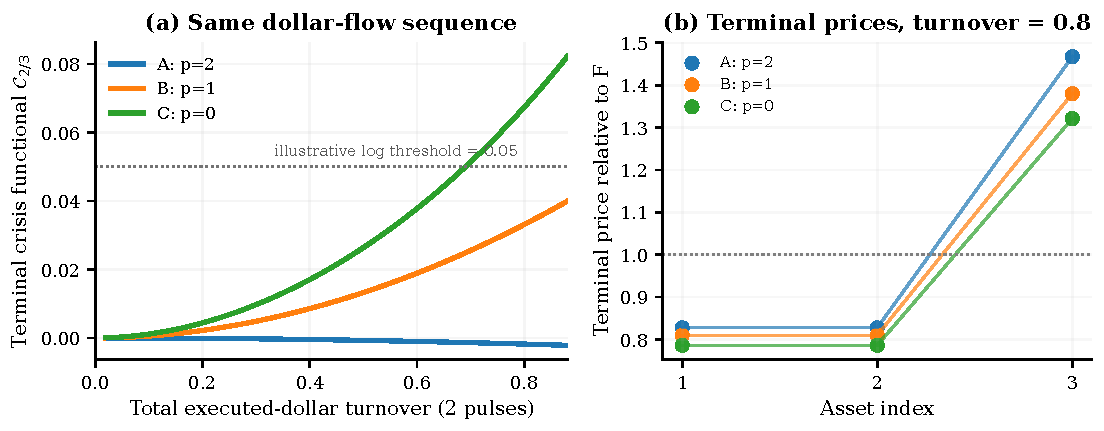
\includegraphics[width=0.98\linewidth]{../../paper/figures/abc_control_comparison.pdf}
\caption{\textbf{对 A/B/C 响应函数实行相同的交易实验。} 两个在终端相互抵消的成交美元脉冲作用于 $N=3$ 项资产，其中 $k=2$、$F=\eta=\rho=1$ 及 $T=3$。左：成交金额配对换手增加时测得的\emph{终端}危机泛函；右：相同总换手 $M=0.8$ 下的终端价格。这一局部示例不同于严重崩盘的存在性构造。虚线阈值用于说明，未经校准。}\label{fig:abcnum}
\end{figure}

\FloatBarrier
\subsection{要求所有资产下跌时的锐界}\label{sec:allcoverage}
市场 C 依赖 $k<N$。为说明覆盖广度条件不仅是一项技术假设，保持\emph{相同的恒定冲击响应}，但将目标改为 $k=N$。此时不存在不达标资产来补偿其余 $N-1$ 项终端损失。模型此时给出精确的、依赖期限的上限，而非任意严重程度构造；即使尚未施加固定执行预算，也已如此。

\begin{theorem}[全资产期限阈值的锐界]\label{thm:critical}
在假设~\ref{asmp:model} 下，令 $g(S)=\eta$ 及 $k=N$，定义
\begin{equation}\label{eq:critical}
\boxed{\delta_{\mathrm{crit}}(N,T)=
\log\frac{\sqrt N}{1+(\sqrt N-1)e^{-\rho T}}.}
\end{equation}
对每个 $\delta\in(0,\delta_{\mathrm{crit}}(N,T))$，都有某个容许终点净成交金额闭合控制，在有限换手及充分大但有限的库存下达到 $\Cris_1(T)\ge\delta$。若 $\delta\ge\delta_{\mathrm{crit}}(N,T)$，则不存在这样的正价格路径。因此，$\delta_{\mathrm{crit}}$ 是所有资产共同对数回撤的\emph{未取到上确界}。
\end{theorem}
\begin{proof}[证明概要]
令 $R(t)^2=\sum_iS_i(t)^2$。在恒定响应下，任何成交金额配对交易均满足 $\dd R^2|_{\rm trade}=2\eta\sum_i\dd X_i=0$。交易间，
\[
\dot R=-\rho\left(R-F\frac{\sum_iS_i}{R}\right).
\]
对于正价格，$\sum_iS_i/R>1$，故 $R(T)>F\{1+(\sqrt N-1)e^{-\rho T}\}$。若每项资产终价均低于 $Fe^{-\delta}$，则 $R(T)\le F\sqrt Ne^{-\delta}$，证明必要性。为证明充分性，将价格向量依次旋转至 $N$ 个仅有一个高坐标的正球面方向，为各资产分配相同恢复权重。每次重新定向都是零和成交金额配对脉冲，恢复阶段的成对控制保持方向固定。相同终价与相同恢复积分，加上 $\sum_iX_i(T)=0$，给出 $X_i(T)=0$，对每个 $i$ 均成立。使正的低坐标趋向零，便可连续逼近该界。完整构造性证明见附录~\ref{app:sharp}。
\end{proof}


\section{需要多少交易？}\label{sec:budget}
迄今的分类回答市场\emph{是否}允许某损失状态。然而，即使市场中该状态可行，参与者拥有的资源也未必足以到达。因此，我们从价格状态几何转向第二道筛选：\emph{达到指定覆盖广度与严重程度，必须成交多少美元换手、卖出多少股？} 以下界适用于一般正响应，是对 A/B/C 可达性结果的补充而非替代。

\begin{theorem}[执行资源下界]\label{thm:resource}
假设容许终端路径满足 $\Cris_\alpha(T)\ge\delta>0$。记 $k=\lceil\alpha N\rceil$ 及 $s=Fe^{-\delta}$。除 $\Phi$ 外，定义单调股数响应坐标 $\Psi(S)=\int_F^S\dd u/g(u)$。则必要美元换手及总卖出股数界恰为到 $s$ 的相应坐标距离：
\begin{equation}\label{eq:resource-lower}
\boxed{M\ge -k\Phi(s)=k\int_s^F\frac{u}{g(u)}\dd u,\qquad
\sum_iH_i^-\ge -k\Psi(s)=k\int_s^F\frac{\dd u}{g(u)}.}
\end{equation}
此外，若 $X_i(T)=0$、禁止卖空，且任一达标资产初始库存不超过 $H_i$，则
\begin{equation}\label{eq:share-bound}
\boxed{\int_s^F\frac{F-u}{g(u)}\dd u\le FH_i.}
\end{equation}
这些不等式是必要而非充分条件，且未必为锐界。
\end{theorem}
\begin{proof}
对于终端达标资产，终价至多为 $s<F$。两个变换坐标都随价格递增，恢复则使它们趋向 $F$ 处的零值。因此，累计负成交美元变差和股数变差必须分别至少为 $-\Phi(s)$ 与 $-\Psi(s)$。对 $k$ 项不同达标资产求和即证明 \eqref{eq:resource-lower}，因为每笔成对成交在跨资产卖出中恰计一次。式~\eqref{eq:share-bound} 则由 \eqref{eq:cost} 右侧非负得到，此时 $X_i(T)=0$ 且 $\theta_i(0)-\theta_i(T)\le H_i$。详细变差论证见附录~\ref{app:accounting}。
\end{proof}

资源界是两个单调坐标中的几何距离，并非最优交易安排。交易方向、恢复时间及接收资产买入容量提出额外要求；下面转向这些执行限制。

若通过\emph{复制相同市场深度}增加 $N$，并固定 $\alpha,\delta$，则 $k=\Theta(N)$，且只要目标可达，\eqref{eq:resource-lower} 就蕴含 $M_*^{\rm end}=\Omega(N)$。这并非适用于真实交易所的普遍市值缩放规律：在此实验中增加 $N$ 也增加总深度。

低价格积分区分不同种类的资源稀缺：
\begin{equation}\label{eq:lowprice}
\int_0^F\frac{u}{g(u)}\dd u,\qquad
\int_0^F\frac{\dd u}{g(u)}.
\end{equation}
对于局部幂律 $g(u)\asymp u^p$，美元积分仅当 $p<2$ 时收敛，股数积分仅当 $p<1$ 时收敛。这些积分准则将资源可行性与可达性的结构和动态条件分离。


\section{有限交易速率与每日价格限制}\label{sec:rateband}
结构上可达的损失可能要求无法以有限速度完成的交易。因此，我们用毛成交股数速率和单时段价格区间限制控制集。这些限制保留屏障定理，而正可达性需要新的连续构造，不能直接使用市场 C 的脉冲控制。

有限执行速度的施加以 Yang~\citep{Yang2019} 等速率受限交易模型为基础；我们的目标仍是共同损失阈值的可达性，而非主体执行目标的最优值。

\subsection{两项独立执行限制}
对于绝对连续非负成交金额配对边速率 $\dot z_e(t)$，定义资产的\emph{毛成交股数速率}为
\begin{equation}\label{eq:grossrate}
 r_i^{\mathrm{gross}}(t)=\frac{1}{S_i(t)}\sum_e |B_{ie}|\dot z_e(t),\qquad
 0\le r_i^{\mathrm{gross}}(t)\le\bar v,\qquad i=1,\ldots,N.
\end{equation}
该界在净额抵消\emph{之前}计算买卖成交。特别地，$|\dot\theta_i|\le r_i^{\mathrm{gross}}\le\bar v$，且不允许 Dirac 型交易。若仅约束带符号净股数速率，则会允许任意规模的同时反向总成交，而无法约束实际换手。

独立地，一项简化的\emph{单时段价格限制规则}要求每个成交价格满足
\begin{equation}\label{eq:band}
 F(1-\beta_-)\le S_i(t)\le F(1+\beta_+),\qquad
 0<\beta_-<1,\quad\beta_+>0.
\end{equation}
控制必须使价格路径保持在该区间内；将越过限制的尝试交易是\emph{不容许的}，而非机械反射回区间。式~\eqref{eq:band} 是一种抽象：东京证券交易所（TSE）的价格限制主要是基于前收盘价或基准价的绝对日元区间，随价格水平变化，并可能跨时段扩大 \citep{JPX2026}。我们不建模未成交订单排队、特别报价、触限集合竞价分配或次日重新开盘。

\begin{proposition}[速率与价格区间排除证书]\label{prop:rate-band}
假设共同冲击函数为正，且在整个容许价格区域内 $g(S)\le G$。在上限~\eqref{eq:grossrate} 下，每项资产均满足
\begin{equation}\label{eq:rate-floor}
 S_i(t)\ge F-\frac{G\bar v}{\rho}(1-e^{-\rho t}),\qquad 0\le t\le T.
\end{equation}
再施加价格区间~\eqref{eq:band}，令
\begin{equation}\label{eq:twofloors}
 S_{\rm floor}=\max\!\left\{F(1-\beta_-),\;F-\frac{G\bar v}{\rho}(1-e^{-\rho T})\right\}>0.
\end{equation}
则对任意覆盖广度 $\alpha$ 和任意容许控制，
\begin{equation}\label{eq:constrained-crisis}
\boxed{\ \mathcal C_\alpha(t)\le \log\frac{F}{S_{\rm floor}}\quad\hbox{for all }t\le T.\ }
\end{equation}
特别地，到达阈值 $\delta>0$ 的一个必要有限速度条件为
\begin{equation}\label{eq:min-speed}
\boxed{\ \bar v\ge\frac{\rho F(1-e^{-\delta})}{G(1-e^{-\rho T})}.\ }
\end{equation}
单时段价格下限独立排除任何 $\delta> -\log(1-\beta_-)$。这些是\emph{必要}约束，通常并非锐的可达性阈值。作为比较，若\emph{假设的}多时段制度按每次前收盘价重设比例下限，则在 $D$ 个时段上的基本界仅为
$S_i(T_D)\ge F\prod_{d=1}^D(1-\beta_{-,d})$ 及
$\mathcal C_\alpha(T_D)\le-\sum_{d=1}^D\log(1-\beta_{-,d})$。
因此，每日价格区间不能解释为以固定基准永久禁止累计崩盘。实际 TSE 限制是按价格分档的日元规则，而非这种比例重设。
\end{proposition}
\begin{proof}
对 $\dot S_i=-\rho(S_i-F)+g(S_i)\dot\theta_i$ 利用常数变易公式及 $|\dot\theta_i|\le\bar v$ 得到 $S_i(t)\ge F-G\bar v\int_0^t e^{-\rho(t-s)}\dd s$，从而证明 \eqref{eq:rate-floor}。价格区间给出第二个下限；每项个体对数损失至多为 $\log(F/S_{\rm floor})$，其横截面平均、覆盖广度分位阈值及两者的最小值同样如此。将仅由速率导出的下限整理，即得到个体损失达到 $\delta$ 的必要条件。
\end{proof}

逐资产比较控制单一价格能够移动的距离。但我们的危机泛函要求许多价格共同移动，且交易协议计算\emph{成对}美元。因此，换手与终点净成交金额闭合协议给出两个额外证书，将相同损失阈值转换为全市场执行要求。由于每笔配对交易的美元金额在毛成交股数核算中对应买卖两侧，因而计入两次，
\begin{equation}\label{eq:rate-turnover}
 M=\frac12\int_0^T\sum_i S_i(t)r_i^{\mathrm{gross}}(t)\dd t
 \le\frac{NF(1+\beta_+)\bar v T}{2}.
\end{equation}
结合定理~\ref{thm:resource}，得到必要的联合约束
\begin{equation}\label{eq:rate-budget-lower}
 \boxed{\ \bar v\ge\frac{2k}{NF(1+\beta_+)T}
 \int_{Fe^{-\delta}}^F\frac{u}{g(u)}\dd u.\ }
\end{equation}
对于闭合成交美元账簿，非负成本恒等式~\eqref{eq:cost} 还给出
\begin{equation}\label{eq:rate-energy}
 E(S_i(T))\le F\bar v T,\qquad
 \bar v\ge \frac{E(Fe^{-\delta})}{FT}
 \quad \hbox{for every qualifying asset.}
\end{equation}
界~\eqref{eq:min-speed}、\eqref{eq:rate-budget-lower} 和 \eqref{eq:rate-energy} 是不同的必要检验；满足它们并不构成危机路径。

朴素的逐资产速率限制似乎只会产生系统性损失的一阶 $O(\bar v)$ 限制。成交金额配对更强：在低速率下，不同资产的领先阶变动在\emph{市场平均}中相互抵消。因此，下面恒定冲击结果是二次而不仅是线性，且自然应与小幅连续构造比较。

\begin{theorem}[恒定冲击下的二次低速率危机屏障]\label{thm:quadratic-rate}
令 $g(S)\equiv\eta>0$，假设成交金额配对 $\sum_iS_i\dot\theta_i=0$，并施加毛成交股数速率上限~\eqref{eq:grossrate}。记 $d_T=1-e^{-\rho T}$ 及
\begin{equation}\label{eq:bsmall}
 b_T=\frac{\eta\bar v}{F\rho}\,d_T<1.
\end{equation}
则无论是否终点净成交金额闭合，对于\emph{每个} $N\ge2$ 与覆盖广度 $\alpha$，
\begin{equation}\label{eq:quadratic-rate}
\boxed{\ \mathcal C_\alpha(T)\le
\left(\frac{\eta\bar v}{F\rho}\right)^2
\left[d_T-\rho T e^{-\rho T}
 +\frac{d_T^2}{2(1-b_T)^2}\right].\ }
\end{equation}
特别地，可能的最大正危机严重程度为 $O(\bar v^2)$（当 $\bar v\downarrow0$ 时）。对固定 $N,T$ 及任意正的价格区间宽度，定理~\ref{thm:finite-rate-construct} 的连续控制\emph{达到此阶}，因此在恒定冲击市场中，其最小所需毛成交速率上限满足 $\bar v_*(\delta)=\Theta(\sqrt\delta)$（当 $\delta\downarrow0$ 时）。隐含系数依赖规定控制，并非精确优化解。
\end{theorem}
\begin{proof}
令 $x_i(t)=S_i(t)-F$ 及 $m(t)=\sum_i x_i(t)$。常数变易公式给出
$|x_i(t)|\le\eta\bar v(1-e^{-\rho t})/\rho$。由于 $\sum_iS_i\dot\theta_i=0$，
$\sum_i\dot\theta_i=-F^{-1}\sum_i x_i\dot\theta_i$，因此
$\dot m=-\rho m-(\eta/F)\sum_i x_i\dot\theta_i$。积分并约束毛成交速率，得到
\begin{equation}\label{eq:meanprice}
\frac{|m(T)|}{NF}\le
\left(\frac{\eta\bar v}{F\rho}\right)^2
 [d_T-\rho T e^{-\rho T}].
\end{equation}
对于 $|x_i(T)|/F\le b_T<1$，Taylor 不等式
$-\log(1+y)\le-y+y^2/[2(1-b_T)^2]$ 蕴含
$\overline L(T)\le |m(T)|/(NF)+b_T^2/[2(1-b_T)^2]$。
利用 $\mathcal C_\alpha\le\overline L$ 得到~\eqref{eq:quadratic-rate}。定理~\ref{thm:finite-rate-construct} 的构造满足 $\mathcal C_1(T)=c_Na^2+O(a^3)$，其中 $c_N>0$，且毛成交速率为 $O(a)$；取 $a\propto\bar v$ 可给出匹配的正 $\Omega(\bar v^2)$ 见证，同时保持固定正宽度的价格区间。这证明所述低速率指数。
\end{proof}

\begin{theorem}[有界连续执行下的正全资产下跌]\label{thm:finite-rate-construct}
假设 $g\in C^3$，此条件在 $F$ 的某邻域上成立，且 $g(F)>0$、$\rho>0$ 及 $e_0=Fg'(F)/g(F)<1$。固定\emph{任意} $N\ge2$、期限 $T>0$、速率上限 $\bar v>0$、单时段区间宽度 $\beta_-,\beta_+>0$，以及每项资产任意固定正数量的初始可用股数。则存在\emph{绝对连续}、成交金额配对、逐资产毛成交速率有界的控制，严格保持在区间内部，对每项资产满足 $X_i(T)=0$，且
\begin{equation}\label{eq:local-speed-crash}
 \boxed{\ S_i(T)<F\ \text{for every }i,\qquad \mathcal C_1(T)>0.\ }
\end{equation}
所达到的损失可以任意小。这\emph{不}意味着在任意严格的上限或区间下，某个指定的固定大阈值仍然可达。
\end{theorem}
\begin{proof}[构造与符号计算]
选择零和向量 $u\in\R^N$，且每个 $u_i\ne0$。令 $\Delta=T/3$、$r=e^{-\rho\Delta}$，并设置有界三段信号
\begin{equation}\label{eq:bounded-control}
 f(t)=
 \begin{cases}
 1,&0\le t<\Delta,\\
 -(1+r),&\Delta\le t<2\Delta,\\
 r,&2\Delta\le t\le T,
 \end{cases}
 \qquad \dot X_i=a u_i f(t).
\end{equation}
美元速率之和为零，且 $\int_0^T f(t)\dd t=0$。
直接积分还给出 $\int_0^T e^{-\rho(T-t)}f(t)\dd t=0$。
记 $h(S)=g(S)/S$ 并展开
$S_i(t)=F+a u_i y(t)+a^2u_i^2 z(t)+O(a^3)$，
其中 $\dot y=-\rho y+h(F)f$、$y(0)=0$，且
$\dot z=-\rho z+h'(F)f y$、$z(0)=0$。
加权抵消蕴含 $y(T)=0$。由于 $h'(F)/h(F)=(e_0-1)/F$，分部积分得到
\begin{equation}\label{eq:finite-rate-coefficient}
 \boxed{\ \log\frac{F}{S_i(T)}=
 \frac{\rho(1-e_0)}{2F^2}\,a^2u_i^2
 \int_0^T e^{-\rho(T-t)}y(t)^2\dd t+O(a^3).\ }
\end{equation}
积分严格为正。因此，对每个充分小的 $a>0$，所有价格均下跌。用总流量最小的非负来源至目标边速率表示每个零和美元速率向量，则 $r_i^{\mathrm{gross}}=|a u_i f|/S_i$。整条价格路径一致收敛至 $F$（当 $a\downarrow0$ 时），因而在 $a$ 充分小时，有限速率上限、价格区间及任意正库存可用量均得到满足。
\end{proof}

该构造补充排除界：在美元闭合条件下，有限速率上限不强制所有终价回到基准。它在限制较大的脉冲控制集的同时，保留局部共同损失的可达性。

\paragraph{分别施加限制后哪些性质仍保留？}
限制容许控制集后，$e(S)\ge2$ 的全局屏障及 $e(S)\ge1$ 的全覆盖排除仍然有效。对于 $p=1$，有界两阶段先买后卖美元速率控制仍使 $k<N$ 项资产终价低于 $F$：每项资产的带符号美元积分为零，同时 $\sum_i S_i(T)=NF$，而 $\log$ 的严格凹性使平均对数损失为正。相比之下，定理~\ref{thm:ABC}(C) 中 $p=0$ 的\emph{任意严重}构造使用瞬时扫单，因此不是~\eqref{eq:grossrate} 下的有效见证。在固定价格区间下，任何单时段终端损失超过 $-\log(1-\beta_-)$ 都在\emph{数学上不可能}。定理~\ref{thm:finite-rate-construct} 证明在两项限制下确实保留的性质：严格为正、但非任意严重的局部全资产下跌。

\begin{table}[H]\centering\small
\caption{不同执行限制如何改变 $p=0$ 构造，其中 $T$ 固定。“局部”表示充分小的正终端全资产损失，并非任意指定的大损失。}
\label{tab:regulatory}
\begin{tabularx}{\linewidth}{@{}p{0.20\linewidth}X X@{}}\toprule
容许控制 & 已证明保留的性质 & 不再能够推断的结论 \\ \midrule
瞬时扫单，无价格区间 & 任意严重的部分覆盖对数损失，$k<N$ & 不刻画有界执行速率 \\
仅限制毛成交速率 $\bar v$ & 任意 $\bar v>0$ 下的局部全资产损失 & 未认证无界严重损失构造 \\
仅施加硬性时段区间 & 区间宽度非零时的局部全资产损失 & $\delta>-\log(1-\beta_-)$ 不可能 \\
两项限制同时施加 & 正上限及正宽度下的局部全资产损失；速率与价格下限证书 & 没有一般精确严重程度阈值或最优执行速率 \\ \bottomrule
\end{tabularx}
\end{table}


\begin{figure}[tbp]\centering
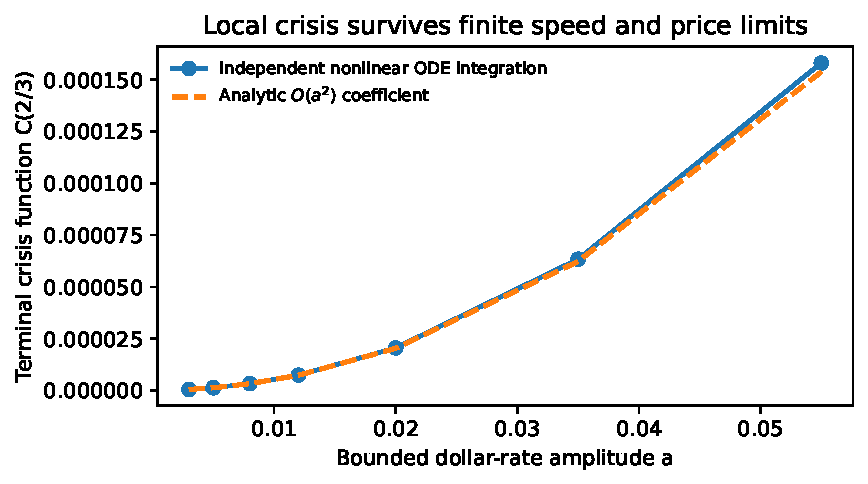
\includegraphics[width=0.76\linewidth]{../../paper/figures/finite_rate_quadratic.pdf}
\caption{\textbf{有限速率控制下的二次局部全资产损失。} 对恒定 $g$ 独立积分得到的非线性价格路径收敛于~\eqref{eq:finite-rate-coefficient} 的解析 $a^2$ 系数。图示幅度充分小，保持价格为正；突出显示的 $a=0.035$ 情形的容许性检查见代码包。}\label{fig:localrate}
\end{figure}


\FloatBarrier
\section{跨时段连续收于跌停价}\label{sec:multiday}
单时段价格下限限制\emph{今日}损失，但下一时段可能从今日更低的收盘价开始。为将上述可达性分析推广至多日，现须跟踪\emph{哪些}资产反复触及下限、危机泛函如何汇总所得损失，以及每笔卖出的对侧是否有足够成交美元容量。这些是相互关联的约束，并非独立示例：目标必须满足覆盖广度阈值，每项目标资产必须以足够速度卖出，其补集则必须在自身速率与区间限制内承接配对流量。

此处\emph{收于跌停价}指最后成交价格等于该时段下限；它不是存在未成交卖单队列的\emph{封死跌停订单簿}。我们的成交交易状态中不含队列动态。解释 Kim 和 Rhee~\citep{KimRhee1997}、Chen 等~\citep{Chen2019} 的价格限制证据时，此区别十分重要。以下从滚动区间的几何上限出发，依次考察条件危机检验、速率、守恒及跨资产容量条件，最后给出经认证的可行路径。

\subsection{滚动区间与精确累计核算}\label{subsec:multiday-protocol}
将交易时间划分为 $D$ 个时段 $[T_{d-1},T_d]$，各自长度为 $\tau_d>0$。隔夜日历时间不计入模型时钟；价格从前收盘价连续延续。在简化的\emph{比例重设}版本中，令 $R_{i,d}=S_i(T_{d-1})$，并要求
\begin{equation}\label{eq:rolling-band}
 (1-\beta_{i,d,-})R_{i,d}\le S_i(t)\le(1+\beta_{i,d,+})R_{i,d},
 \qquad t\in[T_{d-1},T_d],
\end{equation}
其中 $0<\beta_{i,d,-}<1$。收于跌停价表示
$S_i(T_d)=(1-\beta_{i,d,-})R_{i,d}$；连续 $D$ 日跌停指该等式对\emph{相同}资产在 $D$ 个连续时段成立。$k=\lceil\alpha N\rceil$ 项资产连续跌停尚不构成定义~\ref{def:crash} 下的系统性危机：市场平均对数损失也必须达到所选阈值。

对于共同的恒定下限比例 $q=1-\beta_-$，每项连续跌停资产满足
$S_i(T_D)=Fq^D$，损失 $L_i(T_D)=D\lambda$，其中 $\lambda=-\log q$。反之，即便没有连续跌停，在共同区间及相同初始基准价格下，状态约束保证
\begin{equation}\label{eq:rolling-cumulative-upper}
  \Cris_\alpha(T_D)\le D\lambda
\end{equation}
上述结论成立。对于异质区间，右侧可替换为
$\max_i\sum_{d=1}^D[-\log(1-\beta_{i,d,-})]$。这些是\emph{几何上限}，并非成交金额配对路径触及下限的充分条件。

在实际东京证券交易所规则中，每日绝对日元限制取决于基准价所属档位，而非共同百分比，且基准价可以包含特别报价。若基准参考等于前收盘价，则每日收于跌停价对应的概念递推为 $R_{i,d+1}=R_{i,d}-\Delta_-(R_{i,d})$。在指定的连续两个触限时段出现零成交或极少成交后，特别程序可以扩大每日价格区间 \citep{JPX2026}。我们的比例重设模型有意省略这一条件性市场规则。


\subsection{连续跌停收盘下的横截面危机阈值}\label{subsec:multiday-breadth}
第一道门槛来自\emph{定义}。$k$ 只股票连续收于跌停价满足覆盖广度要求，但不自动满足平均损失要求：其余资产在接收配对美元时可能升值。这与允许市场 C 部分覆盖结果的 $k<N$ 补偿机制相同，只是从相反方向观察。以下精确端点恒等式说明，在\emph{不变}泛函下，下跌多数何时构成危机，而暂不构造交易。
\begin{proposition}[条件系统性危机触发检验]\label{prop:multiday-crisis-trigger}
假设相同的 $k=\lceil\alpha N\rceil<N$ 项资产收于 $Fq^D$，此时已历经 $D$ 个相同比例重设时段，其中 $q\in(0,1)$。设其余 $N-k$ 项资产收于 $Y_j>0$，并记 $\lambda=-\log q$。对任意 $0<\delta\le D\lambda$，\emph{终端}危机阈值 $\Cris_\alpha(T_D)\ge\delta$ 成立，当且仅当
\begin{equation}\label{eq:multiday-trigger-product}
\boxed{\qquad \prod_{j=1}^{N-k}\frac{Y_j}{F}
 \le\exp\bigl(kD\lambda-N\delta\bigr).\qquad}
\end{equation}
若其他所有资产的个体对数损失至多为 $D\lambda$（或 $k>N/2$，因此其余 $N-k$ 项资产不足以占据前 $k$ 名），则 $Q_\alpha(T_D)=D\lambda$，且终端危机严重程度精确为
\begin{equation}\label{eq:multiday-trigger-exact}
\boxed{\quad\Cris_\alpha(T_D)=\min\!\left\{D\lambda,
 \frac{kD\lambda-\sum_{j=1}^{N-k}\log(Y_j/F)}{N}\right\}.\quad}
\end{equation}
特别地，仅有一项补偿资产（$k=N-1$）时，其终价必须满足 $Y/F\le\exp(kD\lambda-N\delta)$，才能发生阈值为 $\delta$ 的危机。这些是精确的\emph{条件端点恒等式}，并非存在实现规定收盘价的交易路径的充分条件。
\end{proposition}
\begin{proof}
$k$ 项连续跌停资产的损失为 $D\lambda$，故 $Q_\alpha\ge D\lambda$。对于 $\delta\le D\lambda$，危机准则中的覆盖条件自动满足，剩余要求为 $A\ge\delta$。将终价代入 $A=N^{-1}\sum_i\log(F/S_i)$ 得到 \eqref{eq:multiday-trigger-product}。若其他每项损失均至多为 $D\lambda$，或 $N-k<k$，则第 $k$ 大损失恰为 $D\lambda$，从而证明 \eqref{eq:multiday-trigger-exact}。
\end{proof}
对于命题~\ref{prop:certified-v7} 中经区间认证的 $N=10$、$k=9$、$q=0.97$、$D=2$ 构造，$D\lambda\approx0.060918$。高精度重建中补偿资产收于 $Y/F\approx1.405161$，产生 $\Cris_{0.9}\approx0.020811$。向外舍入证书给出 $1.4047874<Y/F<1.4055543$，从而严格蕴含规定轨迹满足 $\Cris_{0.9}>0.020$。阈值 $\delta=0.020$ 要求 $Y/F\le\exp(9D\lambda-10(0.020))\approx1.416609$，经认证路径满足此条件。因此，接收资产的终价决定相同的广泛连续跌停是否构成系统性损失事件。

\begin{figure}[tbp]\centering
 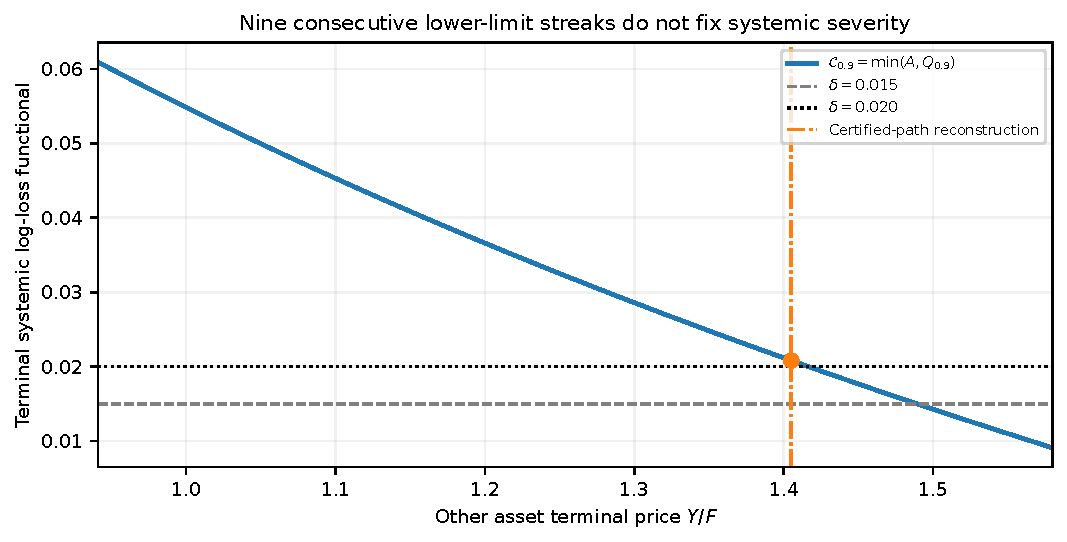
\includegraphics[width=0.85\linewidth]{../../paper/figures/multiday_crisis_trigger.pdf}
\caption{\textbf{仅有连续收于跌停价并不构成系统性危机。} 对 $N=10$，九项资产连续两次收于每日 3\% 跌停价时，条件终端严重程度与其余资产终价的关系。点状标记表示构造出的美元闭合可行路径；1.5\% 和 2.0\% 是对数损失阈值，而非每日价格限制。曲线是代数端点准则，并不声称每个补偿资产价格都在动态上可达。}\label{fig:multiday-crisis-trigger}
\end{figure}

\subsection{连续跌停收盘的最低速度}\label{subsec:multiday-rate}
第二道门槛是\emph{单资产执行容量}。尽管价格向 $F$ 恢复，仍必须在有限时间内达到跌停收盘价。对于 $g(S)\equiv\eta$，设某时段从价格 $s$ 开始、长度为 $\tau$、下限为 $(1-\beta)s$。甚至在询问谁接收配对美元之前，毛成交股数速率上限已通过 $\dot z=-\rho(z-F)-\eta\bar v$、$z(0)=s$ 约束最快下跌。这给出必要阈值，但未解决全市场撮合问题。
\begin{proposition}[滚动价格限制的冲击速率证书]\label{prop:rolling-rate}
在恒定每股冲击模型中，从 $s>0$ 开始的时段若要收于跌停价，必须满足
\begin{equation}\label{eq:single-session-streak-rate}
 \boxed{\quad\bar v\ge \left[\frac{\rho}{\eta}\left(F-s+
 \frac{\beta s}{1-e^{-\rho\tau}}\right)\right]_+.\quad}
\end{equation}
若同一资产在 $D$ 个时段内每次均收于相同比例下限，各时段共同长度为 $\tau$，且 $s_d=Fq^{d-1}$，则
\begin{equation}\label{eq:D-streak-speed}
\boxed{\quad\bar v\ge\frac{\rho F}{\eta}\max_{1\le d\le D}
 \left[1+q^{d-1}\left(\frac{1-q}{1-e^{-\rho\tau}}-1\right)\right].\quad}
\end{equation}
此外，当 $\eta\bar v<\rho F$ 时，所有从 $F$ 出发的价格均遵循永久的\emph{仅由速率导出}的下限 $S_i(t)\ge F-\eta\bar v/\rho$，从而得到必要的整数连续跌停天数界
\begin{equation}\label{eq:streak-D-bound}
\boxed{\quad D\le\frac{\log(1-\eta\bar v/(\rho F))}{\log q}.\quad}
\end{equation}
该界仅在 $\eta\bar v<\rho F$ 时有意义；更大的速率上限不会由此产生有限天数阻碍。这些标量不等式都不是多资产价格区间可行性或终点净成交金额闭合的充分条件。
\end{proposition}
\begin{proof}
常数变易公式与 $\dot\theta_i\ge-\bar v$ 蕴含
$S_i(\tau)\ge F+(s-F)e^{-\rho\tau}-(\eta\bar v/\rho)(1-e^{-\rho\tau})$。
要求 $S_i(\tau)\le(1-\beta)s$ 得到 \eqref{eq:single-session-streak-rate}；逐日代入 $s=Fq^{d-1}$ 得到 \eqref{eq:D-streak-speed}。从初始 $F$ 作同样标量比较给出 $S_i(t)\ge F-(\eta\bar v/\rho)(1-e^{-\rho t})$，进而得到一致下限；将其与 $Fq^D$ 结合，并注意 $\log q<0$，即得 \eqref{eq:streak-D-bound}。
\end{proof}


\subsection{为何全市场连续跌停可能不成立}\label{subsec:multiday-full}
第三道门槛是\emph{全市场守恒}。全资产情形尤其严格：没有补集可以吸收净美元流量。最初产生稳定性屏障的同一势函数，现在在简单的低于基准区间条件下排除第二次同时下跌。这不是独立经济机制，而是 A/B/C 情形已揭示的覆盖广度区别在全局端点的体现。
\begin{theorem}[全资产第二次跌停收盘的阻碍]\label{thm:no-second-global}
假设 $g_i(S)>0$、$\rho_i>0$、基本面基准 $F_i>0$ 不变，并满足资产间瞬时成交美元平衡 $\sum_i\dd X_i=0$。设每项资产在第一时段收于 $S_i(T_1)=q_iF_i<F_i$，且\emph{整个第二时段容许区间}均位于自身基准或以下，
\begin{equation}\label{eq:no-second-condition}
 (1+\beta_{i,2,+})q_i\le1\quad\text{for every }i.
\end{equation}
则不可能\emph{每项}资产在第二时段的收盘价都严格低于第一时段收盘价。特别地，全部 $N$ 项资产不可能在第二日同时收于跌停价。该结论不依赖交易速率上限、终端带符号美元余额或正函数 $g_i$ 的形式。
\end{theorem}
\begin{proof}
采用 $\Phi_i'(S)=S/g_i(S)>0$ 与 $H=\sum_i\Phi_i(S_i)$。交易结算保持 $H$ 不变，恢复贡献为
$\dot H=-\sum_i\rho_i S_i(S_i-F_i)/g_i(S_i)\ge0$，只要所有 $S_i\le F_i$。
条件~\eqref{eq:no-second-condition} 使第二时段完整价格路径保持在此区域内。因此 $H(T_2)\ge H(T_1)$。若第二次收盘价全都低于前收盘价，则所有 $\Phi_i$ 的严格单调性反而给出 $H(T_2)<H(T_1)$，矛盾。
\end{proof}

对于简化的对称比例区间，$q_i=1-\beta_i$ 及
$\beta_{i,2,+}=\beta_i>0$，因此
$(1+\beta_i)(1-\beta_i)=1-\beta_i^2<1$，定理适用。该结论是本\emph{完全成交、跨资产美元平衡、基本面固定}市场的性质，并非预测真实交易所的所有股票不能再次共同下跌：本模型没有未匹配订单、作为外部交易腿的现金及基本面变化。它也不禁止 $k<N$ 项资产连续跌停，同时由其他资产提供抵消美元流量。


同一模型不能表示持续正时间的\emph{全资产封死跌停状态}，其中每个价格固定且严格低于 $F_i$：维持 $\dot S_i=0$ 将要求
每项资产都有 $\dot X_i=\rho_i S_i(S_i-F_i)/g_i(S_i)<0$，与 $\sum_i\dot X_i=0$ 矛盾。触及跌停的收盘成交则允许作为端点条件。持续未匹配卖单队列需要新的订单簿状态，而非简单延长价格轨迹。

\subsection{正的多日资源与核算约束}\label{subsec:multiday-preconditioning}
即使并非所有资产下跌，每项低于 $F$ 的目标资产仍面临向上恢复。因此，终点净成交金额闭合需要路径历史资源，而不只是最终卖出流量：早期高于基准的偏离必须提供正恢复贡献，以补偿后续损失。这是第~\ref{sec:barriers} 节引入的同一势函数的另一种表达，此时积分跨越连续交易时段。
\begin{proposition}[美元闭合连续跌停所需的预处理]\label{prop:streak-precondition}
设某资产从 $F$ 出发，在 $D$ 个时段后以 $s_D<F$ 结束，并满足 $X_i(T_D)=0$。则其轨迹必然在正交易时间测度的集合上到访 $S_i>F$，且满足
\begin{equation}\label{eq:streak-excursion}
 \rho\int_0^{T_D}\frac{S_i(t)(S_i(t)-F)}{g(S_i(t))}\dd t
 =\int_{s_D}^{F}\frac{u}{g(u)}\dd u>0.
\end{equation}
若第一时段之后的每个时段均使该资产保持在 $F$ 或以下，且第一时段上限为 $U_1>F$，则必要条件为
\begin{equation}\label{eq:streak-precondition}
 \boxed{\quad \rho\tau_1\max_{F\le u\le U_1}\frac{u(u-F)}{g(u)}
 \ge \int_{s_D}^{F}\frac{u}{g(u)}\dd u.\quad}
\end{equation}
对于恒定冲击 $g=\eta$，且 $s_D=Fq^D$、$U_1=F(1+\beta_+)$，简化为
$\rho\tau_1\ge(1-q^{2D})/[2\beta_+(1+\beta_+)]$。
记 $H_+=\rho\tau_1\beta_+(1+\beta_+)$，只要 $2H_+<1$，就产生额外的必要连续跌停长度界
\begin{equation}\label{eq:multiday-preconditioning-D}
\boxed{\quad D\le \frac{\log(1-2H_+)}{2\log q}.\quad}
\end{equation}
该界特定于终点净成交金额闭合及后续时段不存在高于基本面偏离的情形。它不足以产生连续跌停路径。
\end{proposition}
\begin{proof}
在完整期限上积分恒等式 $\dd\Phi(S_i)=\dd X_i-\rho S_i(S_i-F)\dd t/g(S_i)$。由于 $X_i(T_D)=0$ 及 $\Phi(F)=0$，前述恢复积分（包含恢复速率系数）必须等于 $-\Phi(s_D)>0$。轨迹处于 $S_i\le F$ 的任何部分均贡献非正被积函数，因此正部分必须来自 $F$ 以上。若后续时段无法升至 $F$ 以上，所有正贡献都必须在第~1 时段取得，其上确界由 \eqref{eq:streak-precondition} 左侧约束。
\end{proof}


\subsection{多资产执行的必要接收容量界}\label{subsec:multiday-cut}
上述检验分别约束下跌股票或整个市场。二者都未刻画系统性危机中至关重要的中间情形：\emph{大多数}资产下跌，而仅剩少数补集资产结算反向美元。这正是 A/B/C 构造背后的 $k<N$ 情形。结构可达性说明补偿资产可以存在；执行可行性则问\emph{其获准的毛成交股数速率和价格区间能够吸收多少}。我们将资产划分为下跌子集 $J$ 及补集 $J^c$。守恒与逐资产毛成交速率直接限制能够跨越此划分的成交美元数量。这是在节点级毛成交速率上限、没有单独边容量的完全交易图上的\emph{必要子集容量不等式}。该不等式将结构上允许的部分覆盖损失与非下跌资产接收所需成交美元的能力联系起来。
\begin{proposition}[市场割集容量与连续跌停下界]\label{prop:market-cut}
固定非空资产子集 $J$，以 $J^c$ 表示其补集。在成交金额配对执行及逐资产毛成交股数速率上限 $\bar v$ 下，每条容许绝对连续路径对几乎处处 $t$ 满足
\begin{equation}\label{eq:market-cut-instant}
\boxed{\left|\sum_{i\in J}\dot X_i(t)\right|\le
\bar v\min\left\{\sum_{i\in J} S_i(t),\sum_{j\in J^c}S_j(t)\right\}.}
\end{equation}
假设在整个时段 $[T_{d-1},T_d]$ 内，其长度为 $\tau_d$，每项 $i\in J$ 都保持在不变基准 $F_i$ 或以下，最终达到 $s_{i,d}<s_{i,d-1}$。令 $\Phi_i'(S)=S/g_i(S)>0$，并记
\begin{equation}\label{eq:cut-required}
K_{J,d}:=\sum_{i\in J}\big[\Phi_i(s_{i,d-1})-\Phi_i(s_{i,d})\big]>0.
\end{equation}
若 $J^c\ne\varnothing$ 且所有补偿资产在该时段满足 $S_j(t)\le U_{j,d}$，则该时段成对成交美元换手 $M_d$ 与所需毛成交股数速率上限满足
\begin{equation}\label{eq:cut-necessary}
\boxed{M_d\ge K_{J,d},\qquad
\bar v\ge\frac{K_{J,d}}{\tau_d\sum_{j\in J^c}U_{j,d}}.}
\end{equation}
当 $J^c=\varnothing$ 时，假设的全部资产同时严格下跌，不可能在完全低于基准的时段内发生。
\end{proposition}
\begin{proof}
成交金额配对给出 $\sum_{i\in J}\dot X_i=-\sum_{j\in J^c}\dot X_j$。在任一集合内，$|\dot X_i|\le S_i r_i^{\mathrm{gross}}\le S_i\bar v$，证明~\eqref{eq:market-cut-instant}。价格响应坐标满足
$\Delta X_i=\Phi_i(s_{i,d})-\Phi_i(s_{i,d-1})+
\rho_i\int_{T_{d-1}}^{T_d}S_i(S_i-F_i)/g_i(S_i)\dd t$.
对于 $i\in J$，积分非正，故 $\sum_{i\in J}\Delta X_i\le-K_{J,d}$。因此流入 $J^c$ 的净成交美元至少为 $K_{J,d}$。总匹配美元换手必须覆盖该流量，补集的总股数容量则不超过 $\bar v\tau_d\sum_{j\in J^c}U_{j,d}$。这给出~\eqref{eq:cut-necessary}。若 $J^c$ 为空，则不存在反向流量。
\end{proof}
由此可以看出结构与执行论证如何汇合。若 $J^c$ 为空，割集没有接收侧，呼应全资产阻碍。若 $J^c$ 非空，路径虽在结构上允许，仍可能要求超过补集可用容量的速率。这些剩余资产对危机泛函还有第二种相反作用：它们的价格升值可能抵消下跌多数的平均对数损失，正如命题~\ref{prop:multiday-crisis-trigger} 所衡量。因此，可行性\emph{同时}要求充足资金吸收能力及足够的未被抵消平均损失。

对于恒定每股冲击 $g_i\equiv\eta$、$k=|J|$ 项相同跌停资产、初始基准 $F$、共同跌停比例 $q\in(0,1)$，以及 $m=N-k>0$ 项补偿资产（其共同涨幅上限比例为 $\beta_{c,+}$），第 $d$ 日的特殊形式为
\begin{equation}\label{eq:cut-special}
\boxed{\bar v\ge \frac{k}{m}\,
\frac{F\,\big(q^{2(d-1)}-q^{2d}\big)}{2\eta\tau_d(1+\beta_{c,+})^{d}}\quad(d\ge2),}
\end{equation}
前提是全部 $k$ 项目标价格保持低于 $F$，且每项补偿资产的前一参考价已从 $F$ 按规定涨幅上限演变。$k/m$ 乘数明确显示资金瓶颈。这是\emph{必要}条件，并非精确最优值。对于十资产两日示例（$k=9,m=1,q=0.97,\beta_{c,+}=0.25,\tau_d=20$），它仅给出 $\bar v\gtrsim 0.0080$；对这一特定配置，下文更强的系统性二次界更有信息量。

\subsection{经验证的较低速率构造与最小速率双侧括界}\label{subsec:v7-certified}
必要约束并不能建立同时可行性。我们现在认证满足所有约束的\emph{单一路径}。固定 $N=10$，其中九项相同目标资产与一项补偿资产，$F=\eta=1$、$\rho=0.4$、两个长度均为 $20$ 的时段、目标滚动区间 $\pm3\%$、补偿资产区间 $\pm25\%$，并要求每项资产终端闭合 $X_i(40)=0$。目标资产共用一条规定的连续价格路径 $x(t)$；补偿资产遵循由成交金额配对确定的标量非线性常微分方程。因此构造简化为两个价格状态，却认证完整十资产模型的容许集非空，并非对异质参数的一般稳健性。以下分段线性目标路径的非线性补偿动态及执行约束，具有可独立重新运行的定点区间证书。
\begin{proposition}[计算机辅助两日速率证书]\label{prop:certified-v7}
在第~\ref{subsec:v7-certified} 节刚给出的十资产设定（$k=9$、$F=\eta=1$、$\rho=0.4$、$\tau_1=\tau_2=20$、目标区间 $\pm3\%$、补偿区间 $\pm25\%$）中，存在一条连续、绝对连续、完全成交金额配对路径，每项资产的终端带符号美元账簿精确归零，相同九项资产分别收于 $0.97$ 及 $0.9409$，同时
\begin{equation}\label{eq:v7-certified-result}
\boxed{\Cris_{0.9}(40)>0.020,\quad \bar v_{\mathrm{used}}<0.285,\quad M<3,\quad H_i^-<2\quad(1\le i\le10).}
\end{equation}
每个成交价格均保持在自身滚动时段区间内。此处 $M$ 将成对成交美元计入一次，$H_i^-$ 表示总卖出股数，因此每项资产初始持有两股足以避免卖空。
\end{proposition}
\begin{proof}[证明提纲；可复现的验证包络见附录~\ref{app:v7certificate}]
令 $r=23/10$。规定共同目标价格 $x(t)$ 为以下节点的连续分段线性插值
\begin{equation}\label{eq:v7-knots}
(t,x)=(0,1),(r,h),(20-r,h),(20,0.97),(20+r,0.995),(40-r,0.995),(40,0.9409).
\end{equation}
第一平台 $h$ 是精确净美元闭合方程在 $1.02$ 附近的唯一根
\begin{equation}\label{eq:v7-root}
101600000000h^2-97138000000h-6646157699=0,
\quad1.02020225507905<h<1.02020225507908.
\end{equation}
补偿资产 $y(t)$ 是下式的唯一正解
$\dot y=-0.4(y-1)-9u(t)/y$、$y(0)=1$，其中
$u(t)=x(t)[\dot x(t)+0.4(x(t)-1)]$。
十项成交美元流量在每个时刻之和均为零，而精确根方程给出每项目标资产满足 $X_i(40)=0$，因此补偿资产亦然。经验证的区间积分给出
\begin{equation}\label{eq:v7-bounds}
\begin{gathered}
1.2219388<y(20)<1.2225356,\quad
1.4047874<y(40)<1.4055543,\\
\sup_t9|u(t)|/y(t)<0.284481,\\
\int_0^{40}9[u(t)]_+/y(t)\dd t<1.880,\qquad
9\int_0^{40}|u(t)|\dd t<2.984.
\end{gathered}
\end{equation}
目标资产的毛成交速率和总卖出股数更小；逐时段区间包络验证两个滚动区间。$e^{0.2}$ 的精确有理包络验证 $\overline L(40)>0.020$，同时九项目标损失为 $-\log(0.9409)>0.020$，从而证明~\eqref{eq:v7-certified-result}。
\end{proof}
对于这个\emph{固定}的十资产、两日、九项连续跌停资产实例，令 $\bar v_*$ 为\emph{所有}还满足 $\Cris_{0.9}(40)\ge0.020$ 的容许路径所需毛成交速率上限的下确界。全系统二次界~\eqref{eq:quadratic-rate} 对每个 $\bar v\le 0.044$（其中 $F=\eta=1$、$\rho=0.4$、$T=40$）蕴含：
\[
\Cris_{0.9}(40)\le (\bar v/0.4)^2
\left[1+\frac{1}{2(1-\bar v/0.4)^2}\right]
\le \frac{1563441}{79210000}<0.020.
\]
由于~\eqref{eq:quadratic-rate} 右侧关于 $\bar v$ 在 $0.044$ 附近连续，且在该值处严格小于 $0.020$，排除结果延伸至某些高于 $0.044$ 的速率。结合命题~\ref{prop:certified-v7} 的可行构造，得到最小毛成交速率上限的严格但非最优括界：

\begin{equation}\label{eq:v7-rate-bracket}
\boxed{\qquad 0.044<\bar v_*<0.285.\qquad}
\end{equation}
该括界对一个固定市场完成本文的问题链：响应规律允许部分覆盖崩盘；危机定义要求足够平均损失；每日价格限制和毛成交速率约束容许路径；成交金额配对结算约束接收侧；经认证路径确实到达目标。下界与上界见证具有不同逻辑作用。经认证控制给出可行速率上界，二次屏障给出严格下界。确定精确全局最小值仍是一个受约束多日最优控制问题。
\paragraph{敏感性及对称性的作用。}
十资产证书有意将九项相同目标状态简化为一条轨迹。保持\emph{同一} $x(t)$ 及精确目标美元闭合不变，数值敏感性检查将十项资产重新划分为 $k$ 项相同目标与 $10-k$ 项相同补偿资产。其共同补偿价格满足 $\dot y=-0.4(y-1)-[k/(10-k)]u(t)/y$。表~\ref{tab:sensitivity} 说明接收资产数量为何重要：固定 $0.020$ 平均损失目标，在受检情形中仅由 $k=9$ 的规定控制达到。改变 $k$ 也改变覆盖比例 $k/10$；这不是固定 $\alpha=0.9$ 的检验。这\emph{不能}证明对 $k<9$ 不存在重新设计后的可行路径；这些行是高精度常微分方程诊断，不同于 $k=9$ 的区间证书。类似地，对固定 $k=9$ 路径，证书证明在对称补偿区间 $\pm24.7\%$ 下合规，在 $\pm24\%$ 下违规（$t=17.7$ 的价格区间严格低于 $0.76$）。改变区间并未重新运行或优化控制。
\begin{table}[H]\centering\small
\caption{\emph{固定且经认证的目标控制形状}对横截面构成的敏感性。仅 $k=9$ 行经区间认证；其他行使用独立积分的高精度标量常微分方程。共同补偿区间是与\emph{计算所得}路径相容的最小对称每日比例；这些数值是诊断结果，而非优化后的可行性阈值。}\label{tab:sensitivity}
\begin{tabular}{@{}rrrrr@{}}\toprule
目标数 $k$ & 补偿资产数 & $y(40)$ & 平均对数损失 & 计算所需区间 \\\midrule
6 & 4 & 1.08112 & 0.00535 & 4.28\%\\
7 & 3 & 1.12302 & 0.00784 & 6.55\%\\
8 & 2 & 1.20141 & 0.01204 & 10.88\%\\
9 & 1 & 1.40516 & 0.02081 & 24.55\%\\
\bottomrule\end{tabular}
\end{table}

\begin{figure}[H]\centering
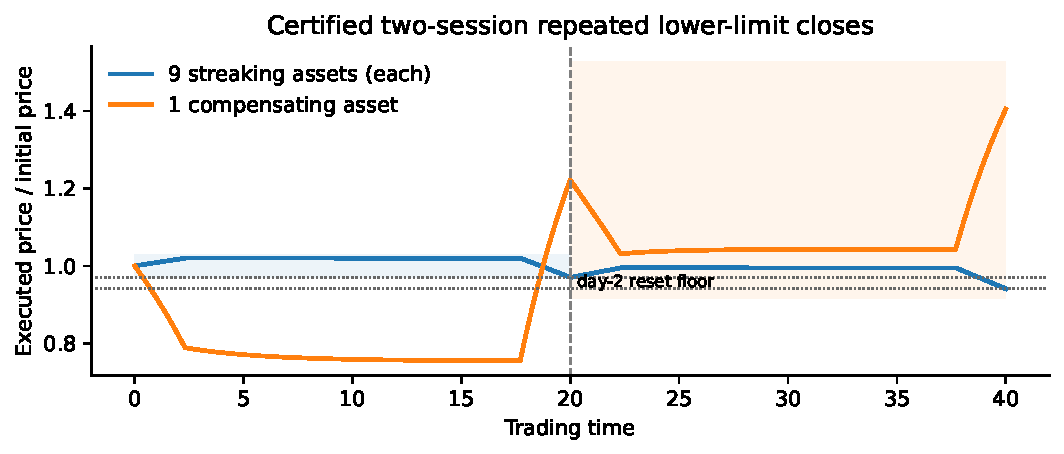
\includegraphics[width=0.87\linewidth]{../../paper/figures/v7_certified_multiday_prices.pdf}
\caption{\textbf{经区间认证的较低速率路径。} 改进两日构造的连续目标与补偿价格。九项目标收于重设后的下限；补偿资产保持在其每日 25\% 限制内。曲线是示意性数值重建；容许性由附录~\ref{app:v7certificate} 所述向外舍入算术独立认证。}\label{fig:v7path}
\end{figure}
\begin{figure}[H]\centering
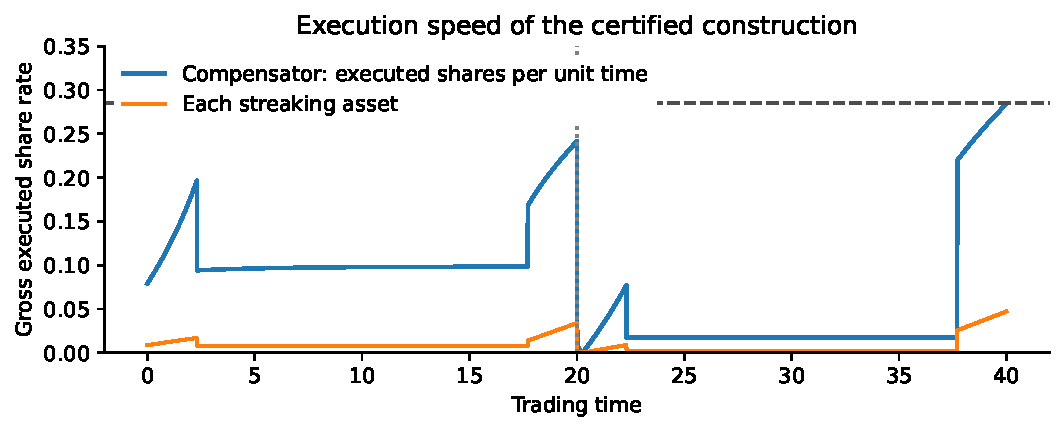
\includegraphics[width=0.87\linewidth]{../../paper/figures/v7_certified_rate_path.pdf}
\caption{\textbf{经认证路径中的毛成交速率。} 计算所得最大毛成交股数速率约为 $0.28422$；严格区间舍入认证其界严格低于 $0.285$，且无瞬时脉冲。上限按资产施加，在买卖净额抵消之前计算。}\label{fig:v7rates}
\end{figure}
\clearpage

\section{解释、局限与可检验含义}\label{sec:discussion}
广义坐标规范形~\eqref{eq:normal-form} 将结果组织成一个序列。成交美元可加地进入，并保持响应适配坐标之和不变；恢复在交易间驱动该总和。曲率产生全局稳定性屏障，A/B/C 函数族说明屏障如何随响应几何变化，坐标距离则约束进入系统性损失集所需的执行资源。有限速率与每日重设区间进一步限制容许路径。经认证两日构造表明这些限制能够同时满足，而子集容量不等式将下跌多数与其余资产的买入容量联系起来。

与均衡驱动机制的区别是明确的。Huang 和 Wang~\citep{HuangWang2009} 研究非同步需求，Cespa 和 Foucault~\citep{CespaFoucault2014} 研究跨资产学习，Cont 和 Wagalath~\citep{ContWagalath2013} 研究困境抛售诱发的相关性，Cordoni 和 Lillo~\citep{CordoniLillo2024} 研究冲击博弈中的策略性不稳定。我们抽去这些选择机制，转而识别在指定\emph{受控市场}中排除危机状态或允许受约束路径到达该状态的条件。Kyle 和 Obizhaeva~\citep{KyleObizhaeva2023} 使用不变性及观测崩盘量化大额交易与执行速度的价格含义；我们的容量与较低速率界不对观测崩盘作经过校准的定量预测。贡献在于共同结算及恢复规则下，结构、资源与执行联合决定的可达性问题，而非替代现有机制。

十资产见证采用对称九目标轨迹与单一补偿资产，将计算化为两个价格状态。表~\ref{tab:sensitivity} 的敏感性检查量化固定目标控制下补偿负担如何变化。经认证事件是一次\emph{系统性回撤}：九只股票在两个时段内各损失 $5.91\%$，第十只升值，等权几何平均价格约下降 $2.06\%$。

实证应用要求从高频数据识别 $g(S)$、恢复 $\rho$、可执行跨资产订单流、库存及现金结算。静态订单簿快照或日频 OHLCV 序列不足以识别这些输入；有效响应 $g$ 并不自动等于 Kyle 的 lambda。构造中的交易所区间是针对\emph{成交价格}的假设百分比限制，实际东京证券交易所通常采用按价格分档的绝对日元区间和规定的扩大规则 \citep{JPX2026}。模型中的跌停收盘并不证明存在未成交卖单队列或真正封死跌停市场。

美元持平再配置可以改变最终持股并耗散交易财富，尽管单独的股数持平往返具有非负执行成本。结果刻画该受控市场的容许价格状态；行为选择及实证事件频率需要进一步模型。

\paragraph{对角冲击与基于势函数的推广。}
本模型的跨资产依赖由成交金额配对产生，边际冲击矩阵则为对角矩阵。在具有直接交叉冲击 $\dd\bm S=\mathsf G(\bm S)\dd\bm\theta$ 且 $\mathsf G$ 可逆的模型中，交易核算提示一形式 $\omega=\one^\top\operatorname{diag}(\bm S)\mathsf G(\bm S)^{-1}\dd\bm S$。标量交易势函数要求该一形式满足适当的恰当性条件，且恢复漂移具有相容符号条件。冲击系数矩阵的对称性或正定性本身不能建立这些性质。这将本文可分离势函数结果与 Alfonsi、Kl\"ock 和 Schied~\citep{AlfonsiKlockSchied2016} 研究的矩阵核条件，以及 Cordoni 和 Lillo~\citep{CordoniLillo2024} 的交叉冲击 Nash 博弈区分开来。

\section{结论}\label{sec:conclusion}
响应适配广义价格坐标将非线性交易冲击化为可加、美元平衡的转移与恢复漂移。其曲率识别全局排除屏障，其坐标距离给出必要资源界。同一响应族呈现三种可达性情形，有界速率、多日区间认证构造表明系统性回撤可以在更严格执行限制下保留。因此，结构可行性、可用资源及多日执行容量构成市场稳定性的连续而数学上不同的检验。

\section*{代码与数值数据可用性}
随附复现包包含 \path{verification/certify_streak_interval.py}（精确有理根隔离与向外舍入定点包络）、\path{verification/verify_consistency.py}、数值敏感性脚本、制图代码、机器可读输出、LaTeX 源码及文件哈希清单。复现命令及软件要求见 \path{REPRODUCE.md}。证书已从源代码重新运行，并通过独立浮点常微分方程及精确有理一致性检查。随稿提供带版本、以校验和索引的复现归档；计算与所提供的源代码及证书版本绑定。

\section*{AI 辅助工具声明}
AI 辅助工具用于起草和组织部分稿件、开发并检查数学计算、编写计算脚本及准备图形。作者对全部内容承担责任，包括数学主张、来源归属及数值证书的可复现性。

\appendix
\section{结算、坐标变换与变差界}\label{app:accounting}
连续响应规则沿有限变差执行路径解释。在理想化脉冲期间，物理时间冻结（$\dd t=0$），状态随执行股数变化而沿响应常微分方程移动。脉冲的成交美元转移是\emph{积分} $\int S_i\dd\theta_i$，而非脉冲起始价格乘以最终股数增量。由 $g>0$ 的连续性，只要中间价格保持为正，就能以容许响应路径连接两个端点。

对于单项资产，微分规则为
\begin{equation}\label{eq:appendix-s}
\dd\theta=\frac{\dd S+\rho(S-F)\dd t}{g(S)}.
\end{equation}
分解 $S=F+(S-F)$ 并积分：
\begin{align*}
\int_0^T S\dd\theta
&=F[\theta(T)-\theta(0)]
+\int_F^{S(T)}\frac{u-F}{g(u)}\dd u
+\rho\int_0^T\frac{(S-F)^2}{g(S)}\dd t,
\end{align*}
其中初始价格为 $F$。这证明 \eqref{eq:cost}。对于 $S<F$，\eqref{eq:E} 中的原函数 $E(S)$ 也非负，因为积分方向反转了负被积函数的符号。因此若 $\theta(T)=\theta(0)$，总执行成本不可能为负。

令 $y=\Phi(S)$ 及 $z=\Psi(S)$，其中
\[
\Phi'(S)=\frac{S}{g(S)},\qquad \Psi'(S)=\frac1{g(S)}.
\]
则
\begin{equation}\label{eq:appendix-yz}
\dd y=\dd X-\rho\frac{S(S-F)}{g(S)}\dd t,
\qquad
\dd z=\dd\theta-\rho\frac{S-F}{g(S)}\dd t.
\end{equation}
恢复项的符号与 $S-F$ 相反。因此，只要 $y<0$（等价于 $S<F$），$y$ 的无交易漂移为正；$z$ 同理。通过分离 \eqref{eq:appendix-yz} 的正负变差，终止于 $y(T)\le\Phi(s)<0$ 的轨迹必须累计至少 $-\Phi(s)$ 的负成交美元变差。一种理解方法是从 $y$ \emph{最后}等于零的时刻开始（若此后不存在零点，则从 $t=0$ 开始）。剩余区间上 $y\le0$ 且恢复漂移非负。因此，负交易变差必须解释至 $y(T)$ 的全部下降。在 $z$ 中作相同论证得到股数卖出界。跨达标资产对卖出求和，使每笔成交金额配对转移恰计一次。若终端达标资产具有库存上限 $H_i$ 且 $X_i(T)=0$，式 \eqref{eq:cost} 蕴含
\[
E(S_i(T))\le F\left[\theta_i(0)-\theta_i(T)\right]\le FH_i.
\]
由于 $E(S)$ 随 $S$ 下降至 $F$ 以下而增加，故 $S_i(T)\le s$ 蕴含 $E(s)\le FH_i$。这证明定理~\ref{thm:resource}。

当 $\rho=0$ 时，$\dd\Phi(S_i)=\dd X_i$。因此终点净成交金额闭合蕴含 $\Phi(S_i(T))=\Phi(F)=0$，结合严格单调性得到 $S_i(T)=F$。在本文可分离响应类中，恢复使非平凡美元闭合端点效应成为可能。

\section{局部双脉冲与三脉冲展开}\label{app:local}
我们记录命题~\ref{prop:two-pulse} 和 \ref{prop:three-pulse} 使用的展开。通过 $x=S/F-1$ 和 $c=g(F)/F^2$ 归一化局部变动。在 $S=F$ 处，成交美元坐标 $y=\Phi(S)$ 满足 $\Phi(F)=0$、$\Phi'(F)=F/g(F)$，且
\begin{equation}\label{eq:local-inverse}
\frac{\dd S}{\dd y}=\frac{g(S)}S,
\qquad
\frac{\dd^2 S}{\dd y^2}=
\frac{g(S)[Sg'(S)-g(S)]}{S^3}.
\end{equation}
因此，记 $e_0=e(F)$，小美元坐标位移 $y$ 后的价格比为
\begin{equation}\label{eq:local-Taylor}
\frac SF=1+cy+\frac12(e_0-1)c^2y^2+O(y^3),
\end{equation}
对处于 $F$ 的某个紧致邻域内的路径，各常数一致有界。

在双脉冲实验中，首个脉冲在零时刻使 $y$ 位移 $hu_i$。它按 \eqref{eq:local-Taylor} 产生初始价格响应。历时 $T$ 的恢复将\emph{价格水平}位移 $S-F$ 乘以 $r=e^{-\rho T}$；终端脉冲从成交美元坐标减去相同美元量 $hu_i$。对 $\Phi$ 和 $\Phi^{-1}$ 作展开，展开中心为 $F$，得到
\begin{align}\label{eq:local-two}
L_i(T)&=c(1-r)hu_i+\frac{c^2h^2}{2}\,\lambda(r,e_0)u_i^2+O(h^3),\\
\frac1N\sum_i L_i(T)&=\frac{c^2h^2}{2N}(1-r)(2-e_0-r)\sum_i u_i^2+O(h^3),\nonumber
\end{align}
其中无需单独给出个体二阶系数 $\lambda$。由于 $\sum_i u_i=0$，线性项在平均中消失。若至少 $k$ 个分量为正，这些资产具有正的一阶损失，且第 $k$ 大损失在 $h$ 很小时为正；在所述时间与曲率条件下，平均损失为正。

在三脉冲实验中，$0,T/2,T$ 的美元坐标脉冲量依次为 $hu_i$、$-(1+r)hu_i$ 和 $rhu_i$，其中 $r=e^{-\rho T/2}$。直接代入并作二阶展开得到
\begin{equation}\label{eq:local-three}
L_i(T)=\frac{1-e_0}{2}c^2h^2u_i^2r(1-r^2)+O(h^3),
\end{equation}
其中一阶项精确抵消。若 $e_0<1$ 且每个 $u_i\ne0$，则充分小的 $h$ 使全部终端损失为正。由于每个脉冲量向量零和，且完整期限内各分量脉冲量相互抵消，构造也满足成交金额配对及终点净成交金额闭合规则。固定 $h$ 时，初始库存要求及换手均有限。

\section{一致资源下的严重部分覆盖回撤}\label{app:severe}
我们构造性证明定理~\ref{thm:ABC}(C)。固定 $N\ge2$，令 $m=N-1$，并选择恒定响应模型 $g(S)=\eta>0$。可以假设目标危机阈值 $\delta$ 较大，因为超过较大阈值的路径自动超过所有较小阈值。只需产生 $m$ 个终价 $\varepsilon\downarrow0$，并以最后一项资产作为“补偿者”，因为每个 $k<N$ 都满足 $k\le m$。

\subsection{成交金额配对交易的径向表示}
对于 $g\equiv\eta$，
\begin{equation}\label{eq:radius-appendix}
\dd(S_i^2)= -2\rho S_i(S_i-F)\dd t+2\eta\dd X_i,
\qquad \one^\top\dd\bm X=0.
\end{equation}
令 $R=(\sum_iS_i^2)^{1/2}$。成交金额配对交易保持 $R$ 固定；固定 $R$ 下的正价格变动可以实现为该球面的严格正坐标区域内的有限变差路径。特别地，在总和相同的两个正向量间对平方价格 $Y_i=S_i^2$ 线性插值：每个中间值 $Y_i>0$，且 $\sum_i\dd Y_i=0$，因此 $\dd X_i=\dd Y_i/(2\eta)$ 是合法成对转移。对应股数增量为 $\dd\theta_i=\dd S_i/\eta$。

选择小常数 $c>0$ 和参数 $b\in(0,\beta)$，其中可取 $\beta=1/5$，使得
\begin{equation}\label{eq:abcs}
a=\sqrt{1-b^2-(m-1)c^2}>b>c>0,
\quad
H=a+(m-1)c+b,
\quad bH<1.
\end{equation}
对于充分小的 $c$，存在这样的选择。在阶段 $j\in\{1,\dots,m\}$，固定球面方向
\begin{equation}\label{eq:uj}
\bm u_j=(c,\ldots,\underbrace{a}_{j},\ldots,c,b),
\qquad \|\bm u_j\|_2=1.
\end{equation}
在整个阶段内令 $\bm S(t)=R(t)\bm u_j$。为使其满足价格方程，采用
\begin{equation}\label{eq:R}
R(t)=F\left[H+(\sqrt N-H)e^{-\rho t}\right],
\qquad
\dot\theta_i=\frac{\rho F}{\eta}\left(u_{j,i}H-1\right).
\end{equation}
事实上，在价格方程中对 $S_i=u_{j,i}R(t)$ 微分，得到 \eqref{eq:R} 及
\begin{equation}\label{eq:dXdt}
\dot X_i=\frac{\rho FR(t)}\eta\,u_{j,i}(u_{j,i}H-1),
\quad \sum_i\dot X_i=\frac{\rho FR(t)}\eta\left(H\sum_i u_{j,i}^2-\sum_i u_{j,i}\right)=0,
\end{equation}
因为 $\sum_i u_{j,i}^2=1$ 及 $\sum_i u_{j,i}=H$。

\subsection{闭合补偿资产美元流量}
在 $t=0$ 从 $F\one$ 开始，并在固定半径 $F\sqrt N$ 上施加正价格脉冲，转至第一方向 $\bm u_1$。使用类似固定半径脉冲在阶段 $\bm u_j$ 间切换。在时刻 $T$ 使用最后一个固定半径脉冲到达
\begin{equation}\label{eq:endpoint-severe}
S_1(T)=\cdots=S_m(T)=\varepsilon,
\quad S_N(T)=\sqrt{R(T)^2-m\varepsilon^2}.
\end{equation}
对于所有充分小的 $\varepsilon$，终端价格向量为正。

对于恒定 $g$，对 \eqref{eq:radius-appendix} 积分得到精确成交美元账簿
\begin{equation}\label{eq:Xledger}
X_i(T)=\frac{S_i(T)^2-F^2}{2\eta}
+\frac\rho\eta\int_0^T S_i(t)[S_i(t)-F]\dd t.
\end{equation}
补偿资产的阶段权重始终为 $b$。定义
\begin{align}\label{eq:compensator}
\mathcal F_\varepsilon(b)=\frac{R_b(T)^2-m\varepsilon^2-F^2}{2\eta}
+\frac\rho\eta\int_0^T bR_b(t)[bR_b(t)-F]\dd t,
\end{align}
其中 $R_b$ 通过 \eqref{eq:R} 连续依赖 $b$。对于充分小的 $c$ 和 $\varepsilon$，有 $\mathcal F_\varepsilon(0)>0$，因为 $R_0(T)>F$。在 $b=\beta$ 处，\eqref{eq:abcs} 给出 $bH<1$，因此时间积分以正比于 $T$ 的速度变负，而终端项保持有界。故存在某个固定且充分长的 $T$，使 $\mathcal F_\varepsilon(\beta)<0$ 对所有小的 $\varepsilon$ 一致成立。由连续性，存在 $b(\varepsilon)\in(0,\beta)$，使 $X_N(T)=0$ 精确成立。

\subsection{闭合每项目标资产美元流量}
剩下需要使其他 $m$ 个终端美元余额相等。资产处于高状态 $a$ 而非低状态 $c$ 时，其恢复被积函数之差为
\begin{equation}\label{eq:W}
W(t)=(a-c)R(t)\big[(a+c)R(t)-F\big].
\end{equation}
此值严格为正：$(a+c)H=1+b(a-b)+mac+bc>1$，且 $R(t)\ge FH$。因此 $W(t)>0$ 对 $t\in[0,T]$ 成立。选择划分 $0=t_0<\dots<t_m=T$，使得
\begin{equation}\label{eq:weights}
\int_{t_{j-1}}^{t_j}W(t)\dd t=\frac1m\int_0^T W(t)\dd t,
\qquad j=1,\ldots,m.
\end{equation}
累计积分连续且严格递增，因而可以作此划分。令目标资产 $j$ 在阶段 $j$ 占据高状态，其余时间占据低状态。所有目标资产具有相同初始价格 $F$、终价 $\varepsilon$，以及 \eqref{eq:Xledger} 中相同恢复积分，故终端余额 $X_i(T)$ 相同。每个脉冲及每个阶段均满足 $\sum_i\dd X_i=0$；由于 $X_N(T)=0$，共同目标余额也必须为零。因此
\begin{equation}\label{eq:allclosed}
X_i(T)=0\qquad\text{for every } i=1,\ldots,N.
\end{equation}

\subsection{一致有限换手与库存}
路径始终处于半径至多为 $F\sqrt N$ 的正球面内，因而全程 $0<S_i\le F\sqrt N$。共有 $m+1=N$ 个固定半径脉冲，每个脉冲可通过平方价格坐标中按分量单调插值实现。因此，累计成交金额配对脉冲换手具有仅依赖 $N,F,\eta$ 的显式但宽松上界。例如，一个安全界为 $N^3F^2/(4\eta)$。在恢复受控阶段，$\sum_i|\dot X_i|/2\le \rho NF^2/\eta$，得到
\begin{equation}\label{eq:uniformM}
M(\gamma)\le M_0:=\frac{N^3F^2}{4\eta}+\frac{\rho NF^2T}{\eta}.
\end{equation}
同样地，$N$ 个脉冲加连续阶段的股数卖出满足
\begin{equation}\label{eq:uniformH}
H_i^-\le H_0:=\frac{NF\sqrt N+\rho FT(\sqrt N+1)}\eta,
\end{equation}
此界独立于 $\varepsilon$。每项资产初始至少持有 $H_0$ 股即可排除卖空。补偿资产价格保持正且有界，其对数损失有限。其余 $m$ 项损失为 $\log(F/\varepsilon)\to\infty$。因此，它们的第 $k$ 阶顺序统计量与平均损失在 $k\le m$ 时都发散。故 $\Cris_\alpha(T)\to\infty$，其中 $M_0,H_0$ 固定有限，证明定理~\ref{thm:ABC}(C)。\qed

\section{证明全覆盖锐界的构造}\label{app:sharp}
必要径向不等式已在定理~\ref{thm:critical} 的证明中建立。以下给出充分性构造。固定 $0<b<1/\sqrt N$，并选择
\begin{equation}\label{eq:fullab}
a=\sqrt{1-(N-1)b^2}>b,
\quad H=a+(N-1)b,
\quad R_b(t)=F\left[H+(\sqrt N-H)e^{-\rho t}\right].
\end{equation}
采用 $N$ 个正单位向量方向，它们由 $(a,b,\ldots,b)$ 排列得到。在零时刻从 $F\one$ 脉冲至 $R_b(0)\bm u_1$，随后沿 $S_i(t)=u_{j,i}R_b(t)$ 演化，使用与 \eqref{eq:R} 相同的成对控制。改变方向时，使用有限的固定半径正平方价格脉冲。在时刻 $T$，作最后一个脉冲，转至等价格点
\begin{equation}\label{eq:fullend}
S_i(T)=\frac{R_b(T)}{\sqrt N},\qquad i=1,\ldots,N.
\end{equation}
为使每项资产的恢复积分相同，定义
\begin{equation}\label{eq:fullW}
W_b(t)=(a-b)R_b(t)\big[(a+b)R_b(t)-F\big].
\end{equation}
此处 $(a+b)H=1+Nab>1$，因此 $W_b(t)>0$ 对 $t\in[0,T]$ 成立。将区间划为 $N$ 部分，使 $W_b$ 的积分相等。每部分中由不同资产充当唯一高价格坐标。全部 $N$ 项资产现具有相同初始价格、相同终价及 \eqref{eq:Xledger} 中相同恢复积分。因此，最终美元余额相同；所有交易均配对，故总和为零，每个余额也精确为零。

当 $b\downarrow0$ 时，\eqref{eq:fullend} 中的共同终价趋向
\[
\frac{F}{\sqrt N}\left[1+(\sqrt N-1)e^{-\rho T}\right],
\]
而 $b\uparrow1/\sqrt N$ 给出 $S_i(T)\to F$。关于 $b$ 的连续性意味着，每个严格介于两者之间的共同终价，均可由正价格、有限换手、完全美元闭合路径到达。对应对数损失范围恰为 $0<\delta<\delta_{\rm crit}(N,T)$，从而完成锐性证明。端点 $\delta_{\rm crit}$ 本身需要含零分量的极限方向，因此被严格正价格要求排除。\qed

\section{有界速率控制：解析细节与审计协议}\label{app:rate}
对于三段控制~\eqref{eq:bounded-control}，恒等式 $\int f=0$ 与 $\int e^{-\rho(T-t)}f(t)\dd t=0$ 由等段宽和几何比例 $r=e^{-\rho T/3}$ 得出。记 $h_0=g(F)/F$ 和 $h_1=g(F)(e_0-1)/F^2$。扰动方程为 $y'=-\rho y+h_0 f$、$z'=-\rho z+h_1fy$。由于 $y(0)=y(T)=0$ 及 $(e^{-\rho(T-t)})'=\rho e^{-\rho(T-t)}$，一次分部积分给出精确恒等式
\begin{equation}\label{eq:ibp}
\int_0^T e^{-\rho(T-t)}f(t)y(t)\dd t
=\frac{\rho}{2h_0}\int_0^T e^{-\rho(T-t)}y(t)^2\dd t.
\end{equation}
所得系数为 $\rho/2$。代入 $h_1/h_0=(e_0-1)/F$ 及 $L_i=-\log(S_i/F)$ 证明~\eqref{eq:finite-rate-coefficient}。在 $p=1$ 时二次系数消失；这与全资产屏障一致，但不排除另一有界信号下的部分覆盖损失。独立验证器直接以美元速率信号积分非线性常微分方程，在净额抵消之前计算毛成交股数，并将有限幅度损失与~\eqref{eq:finite-rate-coefficient} 比较。

严重脉冲见证的高精度重建确认其终端美元核算。有界速率控制构成更严格的容许类，其局部构造与屏障分别建立。

\section{数值实验与可复现性}\label{app:numerics}
本附录记录精确边际价格结算协议下的确定性\emph{构造}价格路径，不模拟订单到达、做市商决策或实际股票数据。对于严重崩盘见证，采用 $g(S)=1$、$F=\eta=\rho=1$。代码选择正价格方向，并数值求解补偿方向与时间划分；切换之间半径及账簿具有解析原函数。在每个交易时刻，成对成交美元总和为零，且到期时\emph{每个}带符号美元账簿在数值精度内闭合。

\begin{table}[H]\centering\small
\caption{若干严重部分覆盖见证。所列换手为可行执行资源，并非未知的最小值。各行均采用目标对数损失 $L=5$，参数归一化为一。}\label{tab:witness}
\begin{tabular}{@{}rrrrrr@{}}\toprule
$N$ & $k$ & $T$ & $\mathcal C_\alpha(T)$ & 换手 $M$ & 最大卖出股数 \\\midrule
3 & 2 & 3 & 3.3168 & 2.6179 & 3.9320\\
12 & 11 & 4 & 4.5781 & 38.6861 & 8.0804\\
20 & 19 & 5 & 4.7477 & 104.1750 & 10.1906\\
\bottomrule\end{tabular}
\end{table}


对于 $N=3$、$k=2$、$T=3$，相同构造给出
\begin{center}\small
\begin{tabular}{@{}rrrr@{}}\toprule
目标对数损失 $L$ & 崩盘泛函 & 可行换手 & 最大股数卖出\\\midrule
$3$ & $1.9845$ & $2.6128$ & $3.9365$\\
 $5$ & $3.3168$ & $2.6179$ & $3.9320$\\
$10$ & $6.6501$ & $2.6179$ & $3.9319$\\
$20$ & $13.3168$ & $2.6179$ & $3.9319$\\
\bottomrule\end{tabular}
\end{center}
绘图实验仅以有限高分辨率采样网格展示连续恢复段；底层分段值及现金流积分均以解析表达式计算，终端闭合则另行检查。对于 $N=12$、$L=5$ 见证，所分发脚本在双精度下的最大终端美元账簿残差小于 $10^{-13}$。数值容差是核算实现正确的证据，不能替代附录~\ref{app:severe} 的构造性证明。

\begingroup\sloppy
使用 \path{verification/finite_rate_and_bands.py} 生成有界速率图；使用 \path{verification/certify_streak_interval.py} 生成两日证书；使用 \path{scripts/improved_multiday_witness.py} 生成数值路径。
图形可通过 \path{scripts/make_figures.py} 及 \path{scripts/make_multiday_figures.py} 重建；检查程序为 \path{verification/verify_consistency.py} 及 \path{scripts/verify_results.py}。
所有图均使用模型生成输入，而非市场观测。\par\endgroup
在仓库根目录运行两次 \texttt{pdflatex} 编译英文原文。


\section{改进两日见证的可复现区间证书}\label{app:v7certificate}
本附录以可独立审计的形式规定计算机辅助证明。代码 \path{verification/certify_streak_interval.py} 使用 Python 整数、有理算术及单位为 $Q=10^{32}$ 的定点区间格式；每次乘除均向外舍入。~\eqref{eq:v7-root} 中 $h$ 的有理端点括区间两端具有严格相反的多项式符号，且多项式在该区间严格递增，因此其中包含唯一相关精确根。

在每个线性目标段内，以局部分段时间写 $x(t)=a+vt$ 及 $u(t)=x(t)[v+\rho(x(t)-1)]$。补偿方程是标量非自治常微分方程 $\dot y=f(t,y):=-\rho(y-1)-9u(t)/y$。在目标斜率变化时刻构成的有限集合之外，其导数为
\[
f_y=-\rho+\frac{9u}{y^2},\qquad f_t=-\frac{9u'}y,\qquad
 y''=f_t+f_y f,\qquad u'=v[v+\rho(2x-1)].
\]
精确目标平台及斜率给出保守整段包络 $|u|<0.107$ 及 $|u'|<0.041$。在自举条带 $0.70\le y\le1.60$ 内，它们蕴含 $|f|<1.70$ 及
\[
|y''|\le\frac{9|u'|}{0.70}
+\left(\rho+\frac{9|u|}{0.70^2}\right)
\left(0.60\rho+\frac{9|u|}{0.70}\right)<5.
\]
在六个目标段中，分别以向外舍入有理算术重新计算最后这个界的更紧值。在步长固定为 $h_0=1/2000$ 的网格上，将标量比较原理与一步 Taylor 包络结合
\[
 y(t+h_0)\in y(t)+h_0 f(t,y(t))+[-B_j h_0^2/2,B_j h_0^2/2],
\]
其中 $B_j$ 为经认证的分段余项界。若起始状态属于 $[l,u]$，标量常微分方程解的比较给出下一步下界 $l+h_0 f(t,l)-B_jh_0^2/2$ 及上界 $u+h_0 f(t,u)+B_jh_0^2/2$，各自向外舍入。局部 $|f|<1.70$ 偏离界包络网格点之间的解，并以归纳方式验证其保持在自举条带内。每个分段线性斜率间断处重新初始化该界，不人为跨越间断迈步。

认证网格步数恰为 $80,000$。对于改进路径，机器可检查输出给出第一日全程 $0.7534859<y(t)<1.223386$，第二日全程 $1.0301664<y(t)<1.406405$。它还包络 $1.2219388<y(20)<1.2225356$ 及
$1.4047874<y(40)<1.4055543$，从而建立第二时段移动的 25\% 限制，以及包含高精度参考值 $1.405160822$ 的终端区间。九项目标资产的坐标沿精确线段演化，每日最低价在规定收盘时达到，每日最高价低于容许上限。步内区间比值同时包络 $|u|/x$ 和 $9|u|/y$，并给出~\eqref{eq:v7-bounds} 中的毛成交速率界。相同包络配合向外舍入时间求和，按所述约束个体总卖出股数及成交美元换手。

最后，终端平均损失为 $-\log[(0.9409)^9 y(40)]/10$。其超过 $0.020$ 的断言在\emph{不}依赖浮点对数的条件下检查：有限有理 Taylor 级数为 $e^{0.2}$ 提供双侧界，并验证 $e^{0.2}(0.9409)^9\sup y(40)<1$。在 $e^{0.21}$ 处的第二个有理检查确认平均损失保持低于 $0.021$。这些断言认证所述分段线性路径及其补偿常微分方程的可行性。

\bibliographystyle{siam}
\bibliography{../../paper/references}

\end{document}
